%% LyX 2.4.1 created this file.  For more info, see https://www.lyx.org/.
%% Do not edit unless you really know what you are doing.
\documentclass[journal,article,submit,pdftex,moreauthors]{Definitions/mdpi}
\usepackage[utf8]{inputenc}
\usepackage{float}
\usepackage{url}
\usepackage{amsmath}
\usepackage{graphicx}

\makeatletter

%%%%%%%%%%%%%%%%%%%%%%%%%%%%%% LyX specific LaTeX commands.

\Title{Utilizing a bounding procedure based on Simulated Annealing to effectively
locate the bounds for the parameters of Radial Basis Function networks}

\TitleCitation{Utilizing a bounding procedure based on Simulated Annealing to effectively
locate the bounds for the parameters of Radial Basis Function networks}

\Author{Ioannis G. Tsoulos$^{1,*}$, Vasileios Charilogis$^{2}$, Dimitrios
Tsalikakis$^{3}$}

\AuthorNames{Ioannis G. Tsoulos, Vasileios Charilogis, Dimitrios Tsalikakis}

\AuthorCitation{Tsoulos, I.G.; Charilogis, V.; Tsalikakis D.}


\address{$^{1}$\quad{}Department of Informatics and Telecommunications,
University of Ioannina, Greece; itsoulos@uoi.gr\\
$^{2}$\quad{}Department of Informatics and Telecommunications, University
of Ioannina, Greece; v.charilog@uoi.gr\\
$^{3}\quad$Department of Engineering Informatics and Telecommunications,
University of Western Macedonia, 50100 Kozani, Greece; tsalikakis@gmail.com}


\corres{Correspondence: itsoulos@uoi.gr}


\abstract{The Radial Basis Function (RBF) networks are an established parametric
machine learning tool, which has been extensively utilized in data
classification and data fitting problems. These specific machine learning
tools have been applied in various scientific areas, such as problems
in physics, chemistry, and medicine, with excellent results. A two-step
technique is usually used to adjust the parameters of these models,
which is in most cases extremely effective. However, it does not effectively
explore the value space of the network parameters and often results
in parameter stability problems. In this paper, the use of a bounding
technique that explores the value space of the parameters of these
networks using intervals generated by a procedure based on the Simulated
Annealing method is recommended. After finding a promising range of
values for the network parameters, a genetic algorithm is applied
within this range of values to more effectively adjust its parameters.
The new method was applied on a wide range of classification and regression
datasets from the relevant literature and the results are reported
in the current manuscript.}


\keyword{Radial Basis Function networks; Simulated Annealing; Stochastic techniques;
Evolutionary Computation}

\newcommand*\LyXZeroWidthSpace{\hspace{0pt}}
\DeclareTextSymbolDefault{\textquotedbl}{T1}
%% Because html converters don't know tabularnewline
\providecommand{\tabularnewline}{\\}
\floatstyle{ruled}
\newfloat{algorithm}{tbp}{loa}
\providecommand{\algorithmname}{Algorithm}
\floatname{algorithm}{\protect\algorithmname}

%%%%%%%%%%%%%%%%%%%%%%%%%%%%%% User specified LaTeX commands.
%  LaTeX support: latex@mdpi.com 
%  For support, please attach all files needed for compiling as well as the log file, and specify your operating system, LaTeX version, and LaTeX editor.

%=================================================================


% For posting an early version of this manuscript as a preprint, you may use "preprints" as the journal and change "submit" to "accept". The document class line would be, e.g., \documentclass[preprints,article,accept,moreauthors,pdftex]{mdpi}. This is especially recommended for submission to arXiv, where line numbers should be removed before posting. For preprints.org, the editorial staff will make this change immediately prior to posting.

%--------------------
% Class Options:
%--------------------
%----------
% journal
%----------
% Choose between the following MDPI journals:
% acoustics, actuators, addictions, admsci, adolescents, aerospace, agriculture, agriengineering, agronomy, ai, algorithms, allergies, alloys, analytica, animals, antibiotics, antibodies, antioxidants, applbiosci, appliedchem, appliedmath, applmech, applmicrobiol, applnano, applsci, aquacj, architecture, arts, asc, asi, astronomy, atmosphere, atoms, audiolres, automation, axioms, bacteria, batteries, bdcc, behavsci, beverages, biochem, bioengineering, biologics, biology, biomass, biomechanics, biomed, biomedicines, biomedinformatics, biomimetics, biomolecules, biophysica, biosensors, biotech, birds, bloods, blsf, brainsci, breath, buildings, businesses, cancers, carbon, cardiogenetics, catalysts, cells, ceramics, challenges, chemengineering, chemistry, chemosensors, chemproc, children, chips, cimb, civileng, cleantechnol, climate, clinpract, clockssleep, cmd, coasts, coatings, colloids, colorants, commodities, compounds, computation, computers, condensedmatter, conservation, constrmater, cosmetics, covid, crops, cryptography, crystals, csmf, ctn, curroncol, currophthalmol, cyber, dairy, data, dentistry, dermato, dermatopathology, designs, diabetology, diagnostics, dietetics, digital, disabilities, diseases, diversity, dna, drones, dynamics, earth, ebj, ecologies, econometrics, economies, education, ejihpe, electricity, electrochem, electronicmat, electronics, encyclopedia, endocrines, energies, eng, engproc, ent, entomology, entropy, environments, environsciproc, epidemiologia, epigenomes, est, fermentation, fibers, fintech, fire, fishes, fluids, foods, forecasting, forensicsci, forests, foundations, fractalfract, fuels, futureinternet, futureparasites, futurepharmacol, futurephys, futuretransp, galaxies, games, gases, gastroent, gastrointestdisord, gels, genealogy, genes, geographies, geohazards, geomatics, geosciences, geotechnics, geriatrics, hazardousmatters, healthcare, hearts, hemato, heritage, highthroughput, histories, horticulturae, humanities, humans, hydrobiology, hydrogen, hydrology, hygiene, idr, ijerph, ijfs, ijgi, ijms, ijns, ijtm, ijtpp, immuno, informatics, information, infrastructures, inorganics, insects, instruments, inventions, iot, j, jal, jcdd, jcm, jcp, jcs, jdb, jeta, jfb, jfmk, jimaging, jintelligence, jlpea, jmmp, jmp, jmse, jne, jnt, jof, joitmc, jor, journalmedia, jox, jpm, jrfm, jsan, jtaer, jzbg, kidney, kidneydial, knowledge, land, languages, laws, life, liquids, literature, livers, logics, logistics, lubricants, lymphatics, machines, macromol, magnetism, magnetochemistry, make, marinedrugs, materials, materproc, mathematics, mca, measurements, medicina, medicines, medsci, membranes, merits, metabolites, metals, meteorology, methane, metrology, micro, microarrays, microbiolres, micromachines, microorganisms, microplastics, minerals, mining, modelling, molbank, molecules, mps, msf, mti, muscles, nanoenergyadv, nanomanufacturing, nanomaterials, ncrna, network, neuroglia, neurolint, neurosci, nitrogen, notspecified, nri, nursrep, nutraceuticals, nutrients, obesities, oceans, ohbm, onco, oncopathology, optics, oral, organics, organoids, osteology, oxygen, parasites, parasitologia, particles, pathogens, pathophysiology, pediatrrep, pharmaceuticals, pharmaceutics, pharmacoepidemiology, pharmacy, philosophies, photochem, photonics, phycology, physchem, physics, physiologia, plants, plasma, pollutants, polymers, polysaccharides, poultry, powders, preprints, proceedings, processes, prosthesis, proteomes, psf, psych, psychiatryint, psychoactives, publications, quantumrep, quaternary, qubs, radiation, reactions, recycling, regeneration, religions, remotesensing, reports, reprodmed, resources, rheumato, risks, robotics, ruminants, safety, sci, scipharm, seeds, sensors, separations, sexes, signals, sinusitis, skins, smartcities, sna, societies, socsci, software, soilsystems, solar, solids, sports, standards, stats, stresses, surfaces, surgeries, suschem, sustainability, symmetry, synbio, systems, taxonomy, technologies, telecom, test, textiles, thalassrep, thermo, tomography, tourismhosp, toxics, toxins, transplantology, transportation, traumacare, traumas, tropicalmed, universe, urbansci, uro, vaccines, vehicles, venereology, vetsci, vibration, viruses, vision, waste, water, wem, wevj, wind, women, world, youth, zoonoticdis 

%---------
% article
%---------
% The default type of manuscript is "article", but can be replaced by: 
% abstract, addendum, article, book, bookreview, briefreport, casereport, comment, commentary, communication, conferenceproceedings, correction, conferencereport, entry, expressionofconcern, extendedabstract, datadescriptor, editorial, essay, erratum, hypothesis, interestingimage, obituary, opinion, projectreport, reply, retraction, review, perspective, protocol, shortnote, studyprotocol, systematicreview, supfile, technicalnote, viewpoint, guidelines, registeredreport, tutorial
% supfile = supplementary materials

%----------
% submit
%----------
% The class option "submit" will be changed to "accept" by the Editorial Office when the paper is accepted. This will only make changes to the frontpage (e.g., the logo of the journal will get visible), the headings, and the copyright information. Also, line numbering will be removed. Journal info and pagination for accepted papers will also be assigned by the Editorial Office.

%------------------
% moreauthors
%------------------
% If there is only one author the class option oneauthor should be used. Otherwise use the class option moreauthors.

%---------
% pdftex
%---------
% The option pdftex is for use with pdfLaTeX. If eps figures are used, remove the option pdftex and use LaTeX and dvi2pdf.

%=================================================================
% MDPI internal commands - do not modify
\firstpage{1} 
 
\setcounter{page}{\@firstpage} 

\pubvolume{1}
\issuenum{1}
\articlenumber{0}
\pubyear{2023}
\copyrightyear{2023}
%\externaleditor{Academic Editor: Firstname Lastname} % For journal Automation, please change Academic Editor to "Communicated by"
\datereceived{}
\daterevised{ } % Comment out if no revised date
\dateaccepted{}
\datepublished{}
%\datecorrected{} % Corrected papers include a "Corrected: XXX" date in the original paper.
%\dateretracted{} % Corrected papers include a "Retracted: XXX" date in the original paper.
\hreflink{https://doi.org/} % If needed use \linebreak
%\doinum{}
%------------------------------------------------------------------
% The following line should be uncommented if the LaTeX file is uploaded to arXiv.org
%\pdfoutput=1

%=================================================================
% Add packages and commands here. The following packages are loaded in our class file: fontenc, inputenc, calc, indentfirst, fancyhdr, graphicx, epstopdf, lastpage, ifthen, lineno, float, amsmath, setspace, enumitem, mathpazo, booktabs, titlesec, etoolbox, tabto, xcolor, soul, multirow, microtype, tikz, totcount, changepage, attrib, upgreek, cleveref, amsthm, hyphenat, natbib, hyperref, footmisc, url, geometry, newfloat, caption

%=================================================================
%% Please use the following mathematics environments: Theorem, Lemma, Corollary, Proposition, Characterization, Property, Problem, Example, ExamplesandDefinitions, Hypothesis, Remark, Definition, Notation, Assumption
%% For proofs, please use the proof environment (the amsthm package is loaded by the MDPI class).

%=================================================================
% The fields PACS, MSC, and JEL may be left empty or commented out if not applicable
%\PACS{J0101}
%\MSC{}
%\JEL{}

%%%%%%%%%%%%%%%%%%%%%%%%%%%%%%%%%%%%%%%%%%
% Only for the journal Diversity
%\LSID{\url{http://}}

%%%%%%%%%%%%%%%%%%%%%%%%%%%%%%%%%%%%%%%%%%
% Only for the journal Applied Sciences:
%\featuredapplication{Authors are encouraged to provide a concise description of the specific application or a potential application of the work. This section is not mandatory.}
%%%%%%%%%%%%%%%%%%%%%%%%%%%%%%%%%%%%%%%%%%

%%%%%%%%%%%%%%%%%%%%%%%%%%%%%%%%%%%%%%%%%%
% Only for the journal Data:
%\dataset{DOI number or link to the deposited data set in cases where the data set is published or set to be published separately. If the data set is submitted and will be published as a supplement to this paper in the journal Data, this field will be filled by the editors of the journal. In this case, please make sure to submit the data set as a supplement when entering your manuscript into our manuscript editorial system.}

%\datasetlicense{license under which the data set is made available (CC0, CC-BY, CC-BY-SA, CC-BY-NC, etc.)}

%%%%%%%%%%%%%%%%%%%%%%%%%%%%%%%%%%%%%%%%%%
% Only for the journal Toxins
%\keycontribution{The breakthroughs or highlights of the manuscript. Authors can write one or two sentences to describe the most important part of the paper.}

%%%%%%%%%%%%%%%%%%%%%%%%%%%%%%%%%%%%%%%%%%
% Only for the journal Encyclopedia
%\encyclopediadef{Instead of the abstract}
%\entrylink{The Link to this entry published on the encyclopedia platform.}
%%%%%%%%%%%%%%%%%%%%%%%%%%%%%%%%%%%%%%%%%%

%%%%%%%%%%%%%%%%%%%%%%%%%%%%%%%%%%%%%%%%%%
% Only for the journal Advances in Respiratory Medicine
%\addhighlights{yes}
%\renewcommand{\addhighlights}{%

%\noindent This is an obligatory section in “Advances in Respiratory Medicine”, whose goal is to increase the discoverability and readability of the article via search engines and other scholars. Highlights should not be a copy of the abstract, but a simple text allowing the reader to quickly and simplified find out what the article is about and what can be cited from it. Each of these parts should be devoted up to 2~bullet points.\vspace{3pt}\\
%\textbf{What are the main findings?}
% \begin{itemize}[labelsep=2.5mm,topsep=-3pt]
% \item First bullet.
% \item Second bullet.
% \end{itemize}\vspace{3pt}
%\textbf{What is the implication of the main finding?}
% \begin{itemize}[labelsep=2.5mm,topsep=-3pt]
% \item First bullet.
% \item Second bullet.
% \end{itemize}
%}
%%%%%%%%%%%%%%%%%%%%%%%%%%%%%%%%%%%%%%%%%%

\makeatother

\begin{document}
\maketitle

\section{Introduction}

A wide range of practical problems can be considered as classification
or regression problems. Such problems occur in areas such as physics
\citep{physics_ml1,physics_ml2}, astronomy \citep{astronomy_ml1,astronomy_ml2},
chemistry \citep{chemistry_ml1,chemistry_ml2}, medicine \citep{med_ml1,med_ml2},
economics \citep{econ_ml1,econ_ml2} etc. A commonly used machine
learning tool used to tackle such problems is the Radial Basis Function
(RBF) network, expressed as the following function:
\begin{equation}
R\left(\overrightarrow{x}\right)=\sum_{i=1}^{k}w_{i}\phi\left(\left\Vert \overrightarrow{x}-\overrightarrow{c_{i}}\right\Vert \right)\label{eq:firstrbf}
\end{equation}
In this equation the following definitions are used for the symbols:
\begin{enumerate}
\item The vector $\overrightarrow{x}$ represents the input pattern with
$d$ number of features.
\item The parameter $k$ stands for the number of weights of the network.
These weights are represented by the values $w_{i},\ i=1,\ldots,k$.
\item The vectors $\overrightarrow{c_{i}},\ i=1,..,k$ represent the the
so - called centers of the network.
\item The function $\phi(x)$ commonly is a Gaussian function with the following
definition:\textbf{ }
\begin{equation}
\phi(x)=\exp\left(-\frac{\left(x-c\right)^{2}}{\sigma^{2}}\right)
\end{equation}
\end{enumerate}
A typical plot of the Gaussian function for $c=0,\ \sigma=1$ is depicted
in Figure \ref{fig:gaussian}. From this graph it is deduced that
the Gaussian RBF decreases regarding the distance from the $c$. The
parameter $c$ and $\sigma$ can be estimated using the K-Means algorithm
introduced by MacQueen \citep{kmeans}. The training error of an RBF
network is defined as:
\begin{equation}
E\left(R\left(\overrightarrow{x}\right)\right)=\sum_{i=1}^{M}\left(R\left(\overrightarrow{x_{i}}\right)-y_{i}\right)^{2}\label{eq:RbfError}
\end{equation}
where $\left(\overrightarrow{x_{i}},y_{i}\right),\ i=1,...,M$ represents
the training set of the objective problem and the values $y_{i}$
are the expected outputs for every pattern $\overrightarrow{x_{i}}$.
\begin{figure}[H]
\begin{centering}
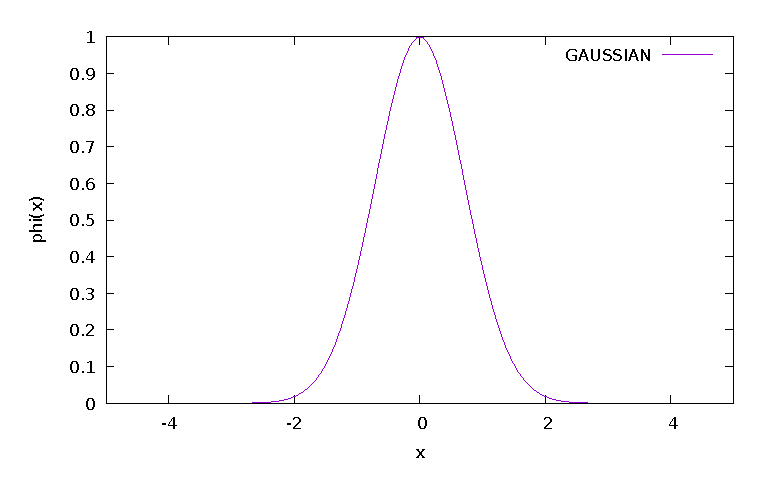
\includegraphics{gaussian}
\par\end{centering}
\caption{A typical plot for the Gaussian function.\protect\label{fig:gaussian}}

\end{figure}
 RBF networks have been incorporated in various cases, such as face
recognition \citep{rbfface}, solutions of differential equations
\citep{rbfde1,rbfde2}, stock prediction \citep{rbfstock}, robotics
\citep{rbfrobotics1,rbfrobotics2}, network security \citep{rbf_dos1,rbf_dos2}
etc. 

Due to the widespread use of these networks, several papers have been
presented in recent years that study their basic characteristics.
For example, Benoudjit et al \citep{rbfkernel} presented a discussion
on kernel widths on RBF networks. Similarly, Oyang et al \citep{rbfkernel2}
presented a novel method for the estimation of the kernel density.
Moreover, Ros et al \citep{rbfinit1} proposed an automatic method
for the initialization of the parameters of RBF networks. Furthermore,
a variety of pruning techniques have also been proposed\textbf{ }\citep{rbfprun1,rbfprun2}
used to reduce efficiently the number of processing units of RBF networks
in order to avoid the overfitting problem. Also, for the effective
training of RBF networks a variety of methods has been proposed in
the recent literature, such as the incorporation of Genetic Algorithms
\citep{rbfga1,rbfga2}, usage of Particle Swam Optimization (PSO)
method \citep{rbfpso1,rbfpso2}, the usage of methods based on Differential
Evolution \citep{rbfdiff1} etc. Furthermore, since there has been
an extremely large spread of parallel programming techniques in recent
decades, publications have also appeared that exploit such techniques
for the efficient and fast training of the above networks \citep{rbfpar1,rbfpar2}.

In most cases, RBF networks are trained using a two-stage technique.
In the first stage, the centers and variances are estimated using
the K-means technique. In the second stage, a linear system is solved
to find the weights of the Gaussian units. Although the above procedure
is extremely fast, it cannot effectively explore the value space for
the network parameters and in many cases numerical stability problems
occur when solving the linear system. This paper proposes a three-stage
method for the efficient training of RBF networks. In the first stage,
an initial estimate of the centers and fluctuations of the RBF network
is made using the K-means technique. Subsequently, an interval generation
method based on Simulated Annealing \citep{siman1} is used to efficiently
identify the optimal interval of network parameter values. The creation
of the value interval is done within a value interval that is based
on the initial estimate of the network parameters made in the first
phase of the method. In the last phase of the proposed technique,
a genetic algorithm is used to train the parameters of the machine
learning model within the optimal value interval resulting from the
second stage of the method.

The rest of this article is divided as follows: in section \ref{sec:Method-description}
the proposed method is presented in detail, in section \ref{sec:Experiments}
the used datasets as well as the conducted experiments are presented
and finally, in section \ref{sec:Conclusions} some conclusions are
discussed as well as some guidelines for improvements of the current
work.

\section{Method description\protect\label{sec:Method-description} }

In this section, a detailed presentation of the three phases of the
proposed technique is made using appropriate algorithms.

\subsection{The first phase of the proposed method }

A typical diagram of an RBF network is depicted in Figure \ref{fig:rbfDiagram}.\textbf{
}Every RBF network with $k$ weights has the following sets of parameters: 
\begin{enumerate}
\item A series of vectors $\overrightarrow{c_{i}},\ i=1,..,k$ that represent
the centers of the network. Each center has $d$ values.
\item Each Gaussian unit has an an additional parameter $\sigma_{i}$, that
corresponds to the variance of this unit.
\item The set of output weights $\overrightarrow{w}$ with $k$ values.
\end{enumerate}
Provided that the input vector $\overrightarrow{x}$ has $d$ values,
the total number of parameters of an RBF network is calculated as:
\begin{equation}
n=(d+2)\times k
\end{equation}
\textbf{ }For the determination of initial values for the centers
and variances the K-means algorithm is utilized here and it is presented
in Algorithm \ref{alg:KMEANS}.

\begin{figure}[H]
\begin{centering}
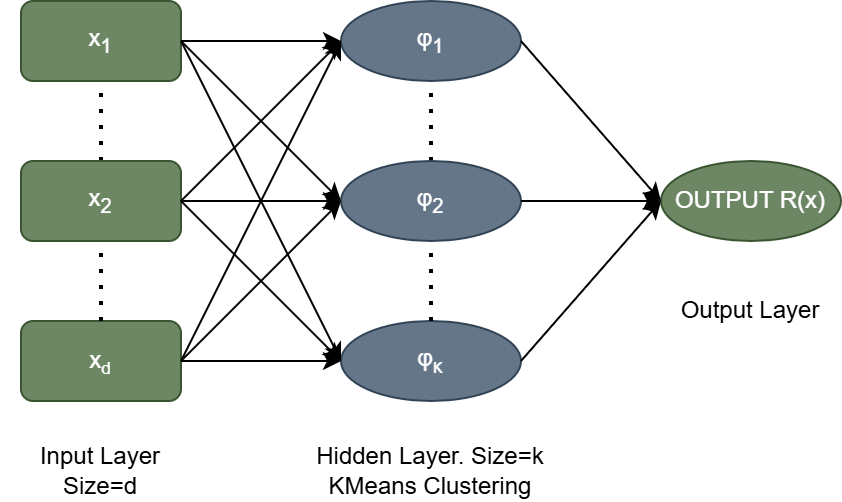
\includegraphics{rbf}
\par\end{centering}
\caption{A typical diagram of an RBF network.\protect\label{fig:rbfDiagram}}

\end{figure}
\begin{algorithm}[H]
\caption{Description of the K-means algorithm.\protect\label{alg:KMEANS}}

\begin{enumerate}
\item \textbf{Initialization}
\begin{enumerate}
\item The input of the algorithm is the points $x_{i},\ i=1,\ldots,M$ belonging
to the train set of the objective problem,
\item \textbf{Define} as $k$ the number of centers.
\item \textbf{Set} $S_{j}=\{\ \}$, $j=1,\ldots,k$.
\end{enumerate}
\item Repeat
\begin{enumerate}
\item \textbf{For} each point $x_{i},\ i=1,...,M$ \textbf{do}
\begin{enumerate}
\item \textbf{Set} $j^{*}=\mbox{argmin}_{m=1}^{k}\left\{ D\left(x_{i},c_{m}\right)\right\} $.
The index $j^{*}$ denotes the nearest center for point$x_{i}$. The
function $D(x,y)$ represents the Euclidean distance.
\item \textbf{Set} $S_{j^{*}}=S_{j^{*}}\cup\left\{ x_{i}\right\} $.
\item \textbf{End For}
\end{enumerate}
\item \textbf{For} every center $c_{j},\ j=1..k$ \textbf{do}
\begin{enumerate}
\item \textbf{Set} $M_{j}$ as the number of points in $S_{j}$
\item \textbf{Update }the center $c_{j}$ with the following equation:
\[
c_{j}=\frac{1}{M_{j}}\sum_{x_{i}\in S_{j}}x_{i}
\]
\end{enumerate}
\item \textbf{End} \textbf{For}
\end{enumerate}
\item The algorithm terminate when $c_{j}$ no longer changes
\item The output of the algorithm are the $\overrightarrow{c_{i}},\ i=1,..,k$
centers and the corresponding variances $\sigma_{i},\ i=1,\ldots,k$
\end{enumerate}
\end{algorithm}
When this process is finished, the vector $\overrightarrow{z}$ with
the calculated parameters is formed with the following procedure:
\begin{enumerate}
\item \textbf{Set} $l=1$
\item \textbf{For} $i=1,\ldots,k$ \textbf{do}
\begin{enumerate}
\item \textbf{For} $j=1,\ldots,d$ \textbf{do} 
\begin{enumerate}
\item \textbf{Set} $z_{l}=c_{i,j}$
\item \textbf{Set} $l=l+1$
\end{enumerate}
\item \textbf{End For}
\end{enumerate}
\item \textbf{End For}
\item \textbf{For} $i=1,\ldots,k$ do
\begin{enumerate}
\item \textbf{Set} $z_{l}=\sigma_{i}$
\item \textbf{Set} $l=l+1$
\end{enumerate}
\item \textbf{End For}
\item \textbf{For} $i=1,\ldots,k$ do
\begin{enumerate}
\item \textbf{Set} $z_{l}=w_{0}$, where $w_{0}$ a positive double precision
number.
\item \textbf{Set} $l=l+1$
\end{enumerate}
\item \textbf{End For}
\end{enumerate}
The layout of the vector $\overrightarrow{z}$ is outlined in Figure
\ref{fig:The-layout-of}. In this layout, the initial values of the
centers are entered at the beginning of the vector, then the initial
values for the variances are entered, and finally the initial values
for the network weights.

\begin{figure}[H]
\caption{The scheme of the particles in the proposed method.\protect\label{fig:The-layout-of}}

$ $
\raggedright{}{\scriptsize{}%
\begin{tabular}{|c|c|c|c|c|c|c|c|c|c|c|c|c|c|c|c|c|c|c|c|c|}
\hline 
{\scriptsize$c_{11}$} & {\scriptsize$c_{12}$} & {\scriptsize ...} & {\scriptsize$c_{1d}$} & {\scriptsize$c_{21}$} & {\scriptsize$c_{22}$} & {\scriptsize ...} & {\scriptsize$c_{2d}$} & {\scriptsize ...} & {\scriptsize$c_{k1}$} & {\scriptsize$c_{k2}$} & {\scriptsize ...} & {\scriptsize$c_{kd}$} & {\scriptsize$\sigma_{1}$} & {\scriptsize$\sigma_{2}$} & {\scriptsize$\ldots$} & {\scriptsize$\sigma_{k}$} & {\scriptsize$w_{1}$} & {\scriptsize$w_{2}$} & {\scriptsize$\ldots$} & {\scriptsize$w_{k}$}\tabularnewline
\hline 
\end{tabular}}{\scriptsize\par}
\end{figure}


\subsection{The second phase of the proposed method }

In the second phase of the algorithm, the value interval for the network
parameters is constructed using a technique based on Simulated Annealing.
The Simulated Annealing is an optimization procedure used in a variety
of cases, such as resource allocation \citep{sa_resource}, portfolio
problems \citep{sa_portfolio}, energy problems \citep{sa_solar},
biology \citep{sa_biology} etc. The algorithm starts from large values
\LyXZeroWidthSpace\LyXZeroWidthSpace of a factor called temperature,
which is gradually decreased. For large values of temperature the
algorithm performs a wide exploration of the search space and at low
values \LyXZeroWidthSpace\LyXZeroWidthSpace it focuses around some
minimum of the objective function. The Simulated Annealing variant
used here minimizes interval functions denoted as: 
\begin{equation}
f\left(x\right)=\left[f_{\mbox{min}}\left(x\right),f_{\mbox{max}}\left(x\right)\right]
\end{equation}
Also, in order to compare two intervals $a=\left[a_{1},a_{2}\right]$
and $b=\left[b_{1},b_{2}\right]$ the operator $D(a,b)$ is incorporated
with the following definition:
\begin{equation}
D(a,b)=\begin{cases}
\mbox{TRUE,} & a_{1}<b_{1}\ \mbox{OR}\ \left(a_{1}=b_{1}\ \mbox{AND}\ a_{2}<b_{2}\right)\\
\mbox{FALSE,} & \mbox{otherwise}
\end{cases}\label{eq:Comparison}
\end{equation}
The method used below assumes that there are value intervals for the
network parameters. The calculation of the functional values \LyXZeroWidthSpace\LyXZeroWidthSpace for
such value intervals is performed using Algorithm \ref{alg:fitness}.
The main steps of the method used in the second phase have as follows:
\begin{enumerate}
\item \textbf{Initialization step}.
\begin{enumerate}
\item \textbf{Construct} the bound vectors $L^{*},\ R^{*}$ using the vector
$\overrightarrow{z}$ of the first phase as follows: 
\[
\begin{array}{ccccc}
L_{i}^{*} & = & -F\times z_{i} & , & i=1,\ldots,n\\
R_{i}^{*} & = & \text{}F\times z_{i} & , & i=1,\ldots,n
\end{array}
\]
\item \textbf{Set $k=0$, $T_{0}>0,\ \epsilon>0,$$r_{T}>0,\ r_{T}<1$}.\textbf{
}The value $T_{0}$ is used to represent the temperature of the algorithm.
\item \textbf{Set }$N_{\mbox{eps}}>0$, which is a positive integer and
it is used as the number of samples that will be created in each iteration
of the algorithm.
\item \textbf{Set} $a>0$ a positive double precision number with the property
$a<1$, that will be used a the perturbation factor for the production
of new samples.
\item \textbf{Set} $N_{s}>0$ a positive integer number.
\item \textbf{Set} $x_{b}=\left[L^{*},R^{*}\right],y_{b}=\mbox{fitness}\left(L^{*},R^{*},N_{s}\right)$.
\item \textbf{Set} $x_{c}=x_{b},y_{c}=y_{b}$
\end{enumerate}
\item \textbf{Main step}.
\begin{enumerate}
\item \textbf{For} $i=1,\ldots,N_{\mbox{eps}}$ \textbf{do}
\begin{enumerate}
\item \textbf{Produce} a random sample $x_{t}=\left(L_{t},R_{t}\right)$
using the procedure of Algorithm \ref{alg:sampling} using as inputs
to the function the interval $x_{c}=\left[L_{c},R_{c}\right]$ and
the double precision number $a$.
\item \textbf{Set} $y_{t}=\mbox{fitness}\left(L_{t},R_{t},N_{s}\right)$.
\item \textbf{If} $D\left(y_{t},y_{c}\right)=\mbox{TRUE}$ \textbf{then}
\textbf{Set} $x_{c}=x_{t},y_{c}=y_{t}$
\item \textbf{Else Set $x_{c}=x_{t}$ }with probability\textbf{ $\min\left\{ 1,\exp\left(-\frac{f_{t}-f_{c}}{T_{k}}\right)\right\} $}
\item \textbf{End if}
\end{enumerate}
\item \textbf{If} $D\left(x_{c},x_{b}\right)=\mbox{TRUE}$ \textbf{then}
\textbf{Set} $x_{b}=x_{c},y_{b}=y_{c}$
\item \textbf{End For}
\end{enumerate}
\item \textbf{Update temperature step}.
\begin{enumerate}
\item \textbf{Set $T_{k+1}=T_{k}r_{T}$}
\item \textbf{Set $k=k+1$.}
\item \textbf{If $T_{k}\le\epsilon$ stop }and\textbf{ return $x_{b}=\left[L_{b},R_{b}\right]$
}as the best located interval of bounds.
\item \textbf{Goto Main Step}.
\end{enumerate}
%
\end{enumerate}
\begin{algorithm}[H]
\caption{The algorithm used to calculate the function value for intervals of
parameters.\protect\label{alg:fitness}}

\textbf{function} fitness$\left(L,R,N_{s}\right)$
\begin{enumerate}
\item \textbf{Create} the set $T=\left\{ r_{1},r_{2},\ldots,r_{N_{s}}\right\} $
with $N_{s}$ random samples in $\left[L,R\right]$.
\item \textbf{Set} $E_{\mbox{min}}=\infty,\ E_{\mbox{max}}=-\infty$
\item \textbf{For} $i=1,\ldots,N_{s}$ \textbf{do}
\begin{enumerate}
\item \textbf{Create} the RBF network $R_{i}\left(\overrightarrow{x}\right)$
using as parameter set the corresponding sample $r_{i}\in T$.
\item \textbf{Calculate} the training error $f_{R_{i}}=\sum_{j=1}^{M}\left(R_{i}\left(\overrightarrow{x_{j}}\right)-y_{j}\right)^{2}$
for the training set of the objective problem.
\item \textbf{If} $f_{R_{i}}\le E_{\mbox{min}}$ \textbf{then} $E_{\mbox{min}}=f_{R_{i}}$
\item \textbf{If} $f_{R_{i}}\ge E_{\mbox{max}}$ \textbf{then} $E_{\mbox{max}}=f_{R_{i}}$
\end{enumerate}
\item \textbf{End For}
\item \textbf{Return} the interval $\left[E_{\mbox{min}},E_{\mbox{max}}\right]$.
\end{enumerate}
\textbf{End function}
\end{algorithm}
\begin{algorithm}[H]
\caption{The sampling function used in the Simulated Annealing algorithm.\protect\label{alg:sampling}}

\textbf{Function} sample$\left(L,R,a\right)$
\begin{enumerate}
\item \textbf{For} $i=1,\ldots,n$ \textbf{do}
\begin{enumerate}
\item \textbf{Set} $m=L_{i}+\frac{R_{i}-L_{i}}{2}$
\item \textbf{Set} $L_{i}^{x}=L_{i}+ar_{1}\left(m-L_{i}\right)$, where
$r_{1}\in[0,1]$ a random value.
\item Set $R_{i}^{x}=R_{i}-ar_{2}\left(R_{i}-m\right)$, where $r_{2}\in[0,1]$
a random value.
\end{enumerate}
\item \textbf{End For}
\item \textbf{Return} $x=\left[L^{x},R^{x}\right]$ the located interval.
\end{enumerate}
\textbf{End function}
\end{algorithm}
The algorithm starts from an initial value interval, which is based
on the result of the first phase of the overall process. At each iteration
it generates random value intervals that are close to the current
value interval. If a value interval with a smaller functional value
than the current one is presented it is accepted, otherwise it will
be accepted with a probability that is high for large temperature
values and decreases significantly as the temperature value drops.
This means that the algorithm makes a wide exploration of the search
space for high temperature values and centers around some minimum
as the temperature value decreases.

\subsection{The final phase of the proposed method}

In the last phase of the proposed procedure, a genetic algorithm is
executed to train the RBF network. The training is performed within
the optimal value interval identified in the previous phase of the
proposed procedure. The main steps of the proposed genetic algorithm
have as follows:
\begin{enumerate}
\item \textbf{Initialization step}.
\begin{enumerate}
\item \textbf{Set} as $N_{g}$ the number of maximum allowed generations
and as $N_{c}$ the number of chromosomes for the genetic population.
\item \textbf{Set} as $p_{s}$ the selection rate with $p_{s}\le1$.
\item \textbf{Set }as $p_{m}$ the mutation rate with $p_{m}\le1$.
\item \textbf{Initialize} the chromosomes $g_{i},\ i=1,\ldots,N_{c}$ as
random vectors inside the bounds $\left[L_{b},R_{b}\right]$ of the
second phase of the suggested algorithm.
\item \textbf{Set} $k=0$
\end{enumerate}
\item \textbf{Fitness calculation step}.
\begin{enumerate}
\item \textbf{For} $i=1,\ldots,N_{c}$ \textbf{do}
\begin{enumerate}
\item \textbf{Create} the RBF network $R_{i}\left(\overrightarrow{x}\right)$using
as parameters the chromosome $g_{i}$.
\item \textbf{Calculate} the corresponding fitness value $f_{i}=\sum_{j=1}^{M}\left(R_{i}\left(\overrightarrow{x_{j}}\right)-y_{j}\right)^{2}$
\end{enumerate}
\item \textbf{End For}
\end{enumerate}
\item \textbf{Genetic operations step}.
\begin{enumerate}
\item \textbf{Selection procedure}. The $p_{s}\times N_{c}$ best chromosomes
with the lowest fitness values are copied intact to the next generation.
The remaining chromosomes will be replaced by new chromosomes produced
in crossover and mutation procedure.
\item \textbf{Crossover procedure}. During the application of crossover,
pairs of chromosomes are chosen from the current population with tournament
selection. For every pair $(z,w)$ of parents two new chromosomes
$\tilde{z}$ and $\tilde{w}$ are will be produced using the following
equations:
\begin{eqnarray}
\tilde{z_{i}} & = & a_{i}z_{i}+\left(1-a_{i}\right)w_{i}\nonumber \\
\tilde{w_{i}} & = & a_{i}w_{i}+\left(1-a_{i}\right)z_{i}\label{eq:crossover_ali-1}
\end{eqnarray}
where $i=1,\ldots,n$ and $a_{i}$ are randomly selected values with
$a_{i}\in[-0.5,1.5]$ \citep{kaelo}. 
\item \textbf{Mutation procedure}. For every element of each chromosome
a random number $r\in[0,1]$ is produced. This element will be altered
randomly when $r\le p_{m}$.
\end{enumerate}
\item \textbf{Termination check step}.
\begin{enumerate}
\item \textbf{Set} $k=k+1$
\item \textbf{If} $k<N_{g}$ \textbf{then} go to Fitness calculation step.
\end{enumerate}
\item \textbf{Testing step}.
\begin{enumerate}
\item \textbf{Obtain} the best chromosome $g_{b}$ from the genetic population,
with the lowest fitness value.
\item \textbf{Create} the corresponding RBF network $R_{b}\left(\overrightarrow{x}\right)$
\item \textbf{Apply} $R_{b}\left(\overrightarrow{x}\right)$ to the corresponding
test set and measure the associated test error.
\end{enumerate}
\end{enumerate}

\section{Experiments \protect\label{sec:Experiments}}

A series of classification and regression datasets from various websites
was incorporate to test the proposed method and to measure its reliability.
The datasets used in the conducted experiments were downloaded from
the following online databases:
\begin{enumerate}
\item The UCI database \url{https://archive.ics.uci.edu/}(accessed on 26
March 2025)\citep{UCL}
\item The Keel website, \url{https://sci2s.ugr.es/keel/datasets.php}(accessed
on 26 March 2025)\citep{Keel}.
\item The Statlib URL \url{ftp://lib.stat.cmu.edu/datasets/index.html }(accessed
on 26 March 2025). 
\end{enumerate}

\subsection{Experimental datasets }

In the conducted experiments the following classification datasets
were used:
\begin{enumerate}
\item The Alcohol dataset, used in various experiments regarding alcohol
consumption \citep{Alcohol}.
\item The Appendicitis dataset \citep{appendicitis}.
\item The Australian dataset, used in various bank transactions \citep{australian}.
\item The Balance dataset, used in a series of psychological experiments
\citep{balance}.
\item The Circular dataset, which is an artificial dataset.
\item The Cleveland dataset, which is a medical dataset \citep{cleveland1,cleveland2}.
\item The Dermatology dataset, obtained from various dermatology problems
\citep{dermatology}.
\item The Hayes roth dataset \citep{hayes-roth}.
\item The Heart dataset, which is a medical dataset regarding heart diseases
\citep{heart}. 
\item The HeartAttack dataset, used in the prediction of heart attacks. 
\item The HouseVotes dataset, that contains data from Congressional voting
in USA \citep{housevotes}.
\item The Ionosphere dataset, obtained from various experiments in the ionosphere
\citep{ion1,ion2}.
\item The Liverdisorder dataset, which is a medical dataset \citep{liver1,liver2}.
\item The Lymography dataset \citep{lymography}.
\item The Mammographic dataset, which is a medical dataset \citep{mammographic}. 
\item The Parkinsons dataset, used for the the detection of Parkinson's
disease \citep{parkinsons1,parkinsons2}.
\item The Phoneme datasets, obtained from various sound experiments.
\item The Pima dataset, a medical dataset used for in the diabetes's disease
\citep{pima}.
\item The Popfailures dataset, related to measurements from climate model
simulations \citep{popfailures}.
\item The Regions2 dataset, which is a medical dataset \citep{regions2}.
\item The Saheart dataset, which is a medical dataset about heart diseases
\citep{saheart}.
\item The Segment dataset, related to issues regarding image processing
\citep{segment}.
\item The Sonar dataset, related to sonar signals \citep{sonar}.
\item The Spiral dataset, which is an artificial dataset.
\item The StatHeart dataset, a medical dataset related to heart diseases.
\item The Student dataset, derived from various experiments in schools \citep{student}.
\item The Transfusion dataset \citep{transfusion}.
\item The WDBC dataset, which is a medical dataset about the detection of
cancer \citep{wdbc}.
\item The Wine dataset, related to the detection of the quality of wines
\citep{wine1,wine2}.
\item The EEG dataset, which is obtained from various EEG measurements \citep{eeg1,eeg2}.
The cases Z\_F\_S, Z\_O\_N\_F\_S, ZO\_NF\_S and ZONF\_S were used
from this dataset.
\item The ZOO dataset, used for animal classification \citep{zoo}.
\end{enumerate}
Moreover, the following regression datasets were obtained for the
conducted experiments:
\begin{enumerate}
\item The Abalone dataset, that contains data related to the age of abalones
\citep{abalone}.
\item The Airfoil dataset, obtained from NASA \citep{airfoil}.
\item The Auto dataset, used to estimate the fuel consumption in cars.
\item The Baseball dataset, related to the estimation of salary of baseball
players.
\item The BK dataset, used for the prediction of points in basketball games
\citep{BK}.
\item The BL dataset, used in some some electricity experiments.
\item The Concrete dataset, derived from civil engineering \citep{concrete}.
\item The Dee dataset, used for the estimation of the price of electricity.
\item The Housing dataset, used to estimate the price of houses \citep{housing}.
\item The Friedman datase\citep{friedman}.
\item The FA dataset, which is related to fat measurements. 
\item The FY dataset, that contains data regarding the fruit flies.
\item The HO dataset, that was derived from the STATLIB repository.
\item The Laser dataset, used in various laser experiments.
\item The MB dataset, derived from the Smoothing Methods in Statistics.
\item The Mortgage dataset, that contains economic measurements.
\item The NT dataset \citep{ntdataset}.
\item The Plastic dataset, that contains measurements form experiments conducted
for the pressure in plastics.
\item The PY dataset \citep{pydataset}.
\item The PL dataset, downloaded from the STATLIB repository.
\item The Quake dataset, related to the estimation of the strength of earthquakes. 
\item The SN dataset, that contains measurements about trellising and pruning.
\item The Stock dataset, which is an economic dataset about the prediction
of the price of stocks.
\item The Treasury dataset, which contains economic measurements. 
\end{enumerate}

\subsection{Experimental results}

The code used in the experiments was implemented in the C++ programming
language and a machine equipped with 128GB RAM running Debian Linux
was utilized in the conducted experiments. Each experiment was executed
30 times and the average classification error was measured for the
classification datasets and the average regression error was measured
for the regression datasets. The classification error is computed
using the following equation:
\begin{equation}
E_{C}\left(R(x)\right)=100\times\frac{\sum_{i=1}^{K}\left(\mbox{class}\left(R\left(x_{i}\right)\right)-y_{i}\right)}{K}
\end{equation}
where the set $T=\left\{ x_{i},y_{i}\right\} ,\ i=1,\ldots,K$ stands
for the test set of the current problem and $R(x)$ is the RBF model.
The regression error is calculated through the following equation:
\begin{equation}
E_{R}\left(R(x)\right)=\frac{\sum_{i=1}^{K}\left(R\left(x_{i}\right)-y_{i}\right)^{2}}{K}
\end{equation}
The values for the parameters of the proposed method are mentioned
in Table \ref{tab:settings}. In the following tables that describe
the experimental results the following notation is used:
\begin{enumerate}
\item The column DATASET represents the name of the objective problem.
\item The column BFGS denotes the application of the BFGS optimization method
\citep{powell} in the training of a neural network \citep{nn1,nn2}
with 10 processing nodes.
\item The column ADAM stands for the incorporation of the ADAM optimizer
\citep{adam} to train an artificial neural network with 10 processing
nodes.
\item The column NEAT represents the usage of the NEAT method (NeuroEvolution
of Augmenting Topologies ) \citep{neat}.
\item The column RBF-KMEANS stands for the usage of the original two - phase
method to train an RBF network with 10 processing nodes.
\item The column GENRBF represents the incorporation of the method proposed
in \citep{genrbf} to train an RBF network with 10 processing nodes.
\item The column PROPOSED denotes the usage of the proposed method to train
an RBF network with 10 processing nodes.
\item The row AVERAGE represents the average classification or regression
error.
\end{enumerate}
\begin{table}[H]
\caption{The values for the experimental parameters.\protect\label{tab:settings}}

\centering{}%
\begin{tabular}{|c|c|c|}
\hline 
PARAMETER & MEANING & VALUE\tabularnewline
\hline 
\hline 
$w_{0}$ & Initial values for the weights & 100.0\tabularnewline
\hline 
$F$ & Scale factor used in the initialization & 10.0\tabularnewline
\hline 
$T_{0}$ & Initial temperature & $10^{6}$\tabularnewline
\hline 
$\epsilon$ & Small value used in comparisons & $10^{-6}$\tabularnewline
\hline 
$a$ & Perturbation factor & 0.001\tabularnewline
\hline 
$N_{s}$ & Number of samples used in the fitness calculation & 100\tabularnewline
\hline 
$N_{\mbox{eps}}$ & Number of samples taken in Simulated Annealing & 100\tabularnewline
\hline 
$N_{c}$ & Number of chromosomes & 500\tabularnewline
\hline 
$N_{g}$ & Maximum number of allowed generations & 200\tabularnewline
\hline 
$p_{s}$ & Selection rate & 0.1\tabularnewline
\hline 
$p_{m}$ & Mutation rate & 0.05\tabularnewline
\hline 
\end{tabular}
\end{table}
The results from the application of the previously mentioned machine
learning methods to the classification datasets are depicted in Table
\ref{tab:experClass} and for regression datasets the results are
presented in Table \ref{tab:experRegression}.

\begin{table}[H]
\caption{Experimental results for the classification datasets using the series
of machine learning methods adopted here. The numbers in cells represent
average classification error as measured on the corresponding test
set.\protect\label{tab:experClass}}

\centering{}%
\begin{tabular}{|c|c|c|c|c|c|c|}
\hline 
\textbf{DATASET} & \textbf{BFGS} & \textbf{ADAM} & \textbf{NEAT} & \textbf{RBF-KMEANS} & \textbf{GENRBF} & \textbf{PROPOSED}\tabularnewline
\hline 
\hline 
Alcohol & 41.50\% & 57.78\% & 66.80\% & 49.38\% & 52.45\% & 31.28\%\tabularnewline
\hline 
Appendicitis & 18.00\% & 16.50\% & 17.20\% & 12.23\% & 16.83\% & 15.27\%\tabularnewline
\hline 
Australian & 38.13\% & 35.65\% & 31.98\% & 34.89\% & 41.79\% & 21.00\%\tabularnewline
\hline 
Balance & 8.64\% & 7.87\% & 23.14\% & 33.42\% & 38.02\% & 12.95\%\tabularnewline
\hline 
Cleveland & 77.55\% & 67.55\% & 53.44\% & 67.10\% & 67.47\% & 50.82\%\tabularnewline
\hline 
Circular & 6.08\% & 19.95\% & 35.18\% & 5.98\% & 21.43\% & 4.19\%\tabularnewline
\hline 
Dermatology & 52.92\% & 26.14\% & 32.43\% & 62.34\% & 61.46\% & 36.13\%\tabularnewline
\hline 
Hayes Roth & 37.33\% & 59.70\% & 50.15\% & 64.36\% & 63.46\% & 33.54\%\tabularnewline
\hline 
Heart & 39.44\% & 38.53\% & 39.27\% & 31.20\% & 28.44\% & 15.33\%\tabularnewline
\hline 
HeartAttack & 46.67\% & 45.55\% & 32.34\% & 29.00\% & 40.48\% & 18.52\%\tabularnewline
\hline 
HouseVotes & 7.13\% & 7.48\% & 10.89\% & 6.13\% & 11.99\% & 3.74\%\tabularnewline
\hline 
Ionosphere & 15.29\% & 16.64\% & 19.67\% & 16.22\% & 19.83\% & 7.39\%\tabularnewline
\hline 
Liverdisorder & 42.59\% & 41.53\% & 30.67\% & 30.84\% & 36.97\% & 27.92\%\tabularnewline
\hline 
Lymography & 35.43\% & 29.26\% & 33.70\% & 25.50\% & 29.33\% & 20.64\%\tabularnewline
\hline 
Mammographic & 17.24\% & 46.25\% & 22.85\% & 21.38\% & 30.41\% & 17.21\%\tabularnewline
\hline 
Parkinsons & 27.58\% & 24.06\% & 18.56\% & 17.41\% & 33.81\% & 15.35\%\tabularnewline
\hline 
Phoneme & 15.58\% & 29.43\% & 22.34\% & 23.32\% & 26.29\% & 16.62\%\tabularnewline
\hline 
Pima & 35.59\% & 34.85\% & 34.51\% & 25.78\% & 27.83\% & 23.59\%\tabularnewline
\hline 
Popfailures & 5.24\% & 5.18\% & 7.05\% & 7.04\% & 7.08\% & 4.80\%\tabularnewline
\hline 
Regions2 & 36.28\% & 29.85\% & 33.23\% & 38.29\% & 39.98\% & 25.54\%\tabularnewline
\hline 
Saheart & 37.48\% & 34.04\% & 34.51\% & 32.19\% & 33.90\% & 29.64\%\tabularnewline
\hline 
Segment & 68.97\% & 49.75\% & 66.72\% & 59.68\% & 54.25\% & 40.83\%\tabularnewline
\hline 
Sonar & 25.85\% & 30.33\% & 34.10\% & 27.90\% & 37.13\% & 18.25\%\tabularnewline
\hline 
Spiral & 47.99\% & 48.90\% & 50.22\% & 44.87\% & 50.02\% & 22.52\%\tabularnewline
\hline 
Statheart & 39.65\% & 44.04\% & 44.36\% & 31.36\% & 42.94\% & 19.52\%\tabularnewline
\hline 
Student & 7.14\% & 5.13\% & 10.20\% & 5.49\% & 33.26\% & 5.11\%\tabularnewline
\hline 
Transfusion & 25.84\% & 25.68\% & 24.87\% & 26.41\% & 25.67\% & 24.59\%\tabularnewline
\hline 
Wdbc & 29.91\% & 35.35\% & 12.88\% & 7.27\% & 8.82\% & 5.00\%\tabularnewline
\hline 
Wine & 59.71\% & 29.40\% & 25.43\% & 31.41\% & 31.47\% & 7.71\%\tabularnewline
\hline 
Z\_F\_S & 39.37\% & 47.81\% & 38.41\% & 13.16\% & 23.37\% & 3.16\%\tabularnewline
\hline 
Z\_O\_N\_F\_S & 65.67\% & 78.79\% & 77.08\% & 48.70\% & 68.40\% & 46.77\%\tabularnewline
\hline 
ZO\_NF\_S & 43.04\% & 47.43\% & 43.75\% & 9.02\% & 22.18\% & 3.63\%\tabularnewline
\hline 
ZONF\_S & 15.62\% & 11.99\% & 5.44\% & 4.03\% & 17.41\% & 1.79\%\tabularnewline
\hline 
ZOO & 10.70\% & 14.13\% & 20.27\% & 21.93\% & 33.50\% & 4.50\%\tabularnewline
\hline 
\textbf{AVERAGE} & \textbf{32.98\%} & \textbf{33.60\%} & \textbf{32.46\%} & \textbf{28.39\%} & \textbf{34.64\%} & \textbf{18.67\%}\tabularnewline
\hline 
\end{tabular}
\end{table}
The table \ref{tab:experClass} presents the error rates of various
machine learning models (BFGS, ADAM, NEAT, RBF-KMEANS, GENRBF, PROPOSED)
on different classification datasets. Each row corresponds to a dataset,
while each column represents the error rate of a specific model. These
values indicate the percentage of incorrect predictions, with lower
values reflecting better performance. The last row of the table includes
the average error rates for each model. Statistical analysis of the
data reveals significant insights. The PROPOSED model exhibits the
lowest average error rate (18.67\%) compared to the other models,
establishing it as the optimal choice based on the table. Conversely,
the other models demonstrate higher average error rates, with GENRBF
showing the highest average (34.64\%). Additionally, significant variations
in error rates across datasets are observed. For instance, in the
\textquotedbl Circular\textquotedbl{} and \textquotedbl ZONF\_S\textquotedbl{}
datasets, the PROPOSED model outperforms others with very low error
rates (4.19\% and 1.79\%, respectively). Conversely, in datasets like
\textquotedbl Cleveland,\textquotedbl{} the NEAT model shows a lower
error rate (53.44\%) compared to the PROPOSED model (50.82\%). Notably,
in certain datasets, the performance of the PROPOSED model is significantly
inferior to other models. For example, in the \textquotedbl Alcohol\textquotedbl{}
and \textquotedbl Z\_F\_S\textquotedbl{} datasets, the PROPOSED model
exhibits much higher error rates compared to other models. This indicates
that while the PROPOSED model generally has the lowest average error
rate, its performance may not be consistent across all datasets. In
conclusion, the PROPOSED model emerges as the best general choice
for minimizing error rates, though its evaluation depends on the characteristics
of each dataset. The performance differences among models highlight
the need for careful model selection depending on the application.s
\begin{table}[H]
\caption{Experimental results for regression datasets. Numbers in cells represent
average regression error as calculated on the corresponding test set.\protect\label{tab:experRegression}}

\centering{}%
\begin{tabular}{|c|c|c|c|c|c|c|}
\hline 
\textbf{DATASET} & \textbf{BFGS} & \textbf{ADAM} & \textbf{NEAT} & \textbf{RBF-KMEANS} & \textbf{GENRBF} & \textbf{PROPOSED}\tabularnewline
\hline 
Abalone & 5.69 & 4.30 & 9.88 & 7.37 & 9.98 & 5.10\tabularnewline
\hline 
Airfoil & 0.003 & 0.005 & 0.067 & 0.27 & 0.121 & 0.004\tabularnewline
\hline 
Auto & 60.97 & 70.84 & 56.06 & 17.87 & 16.78 & 9.68\tabularnewline
\hline 
Baseball & 119.63 & 77.90 & 100.39 & 93.02 & 98.91 & 86.19\tabularnewline
\hline 
BK & 0.28 & 0.03 & 0.15 & 0.02 & 0.023 & 0.153\tabularnewline
\hline 
BL & 2.55 & 0.28 & 0.05 & 0.013 & 0.005 & 0.0002\tabularnewline
\hline 
Concrete & 0.066 & 0.078 & 0.081 & 0.011 & 0.015 & 0.006\tabularnewline
\hline 
Dee & 2.36 & 0.630 & 1.512 & 0.17 & 0.25 & 0.16\tabularnewline
\hline 
Housing & 97.38 & 80.20 & 56.49 & 57.68 & 95.69 & 18.70\tabularnewline
\hline 
Friedman & 1.26 & 22.90 & 19.35 & 7.23 & 16.24 & 1.45\tabularnewline
\hline 
FA & 0.426 & 0.11 & 0.19 & 0.015 & 0.15 & 0.019\tabularnewline
\hline 
FY & 0.22 & 0.038 & 0.08 & 0.041 & 0.041 & 0.077\tabularnewline
\hline 
HO & 0.62 & 0.035 & 0.169 & 0.03 & 0.076 & 0.01\tabularnewline
\hline 
Laser & 0.015 & 0.03 & 0.084 & 0.03 & 0.075 & 0.003\tabularnewline
\hline 
MB & 0.129 & 0.06 & 0.061 & 2.16 & 0.41 & 5.49\tabularnewline
\hline 
Mortgage & 8.23 & 9.24 & 14.11 & 1.45 & 1.92 & 0.14\tabularnewline
\hline 
NT & 0.129 & 0.12 & 0.33 & 8.14 & 0.02 & 0.007\tabularnewline
\hline 
PL & 0.29 & 0.117 & 0.098 & 2.12 & 0.155 & 0.023\tabularnewline
\hline 
Plastic & 20.32 & 11.71 & 20.77 & 8.62 & 25.91 & 2.29\tabularnewline
\hline 
PY & 0.578 & 0.09 & 0.075 & 0.012 & 0.029 & 0.019\tabularnewline
\hline 
Quake & 0.42 & 0.06 & 0.298 & 0.07 & 0.79 & 0.036\tabularnewline
\hline 
SN & 0.40 & 0.026 & 0.174 & 0.027 & 0.027 & 0.024\tabularnewline
\hline 
Stock & 302.43 & 180.89 & 12.23 & 12.23 & 25.18 & 1.53\tabularnewline
\hline 
Treasury & 9.91 & 11.16 & 15.52 & 2.02 & 1.89 & 0.51\tabularnewline
\hline 
\textbf{AVERAGE} & \textbf{26.43} & \textbf{19.62} & \textbf{12.84} & \textbf{9.19} & \textbf{12.28} & \textbf{5.48}\tabularnewline
\hline 
\end{tabular}
\end{table}

The table \ref{tab:experRegression} displays the absolute error values
resulting from the application of various machine learning models
(BFGS, ADAM, NEAT, RBF-KMEANS, GENRBF, PROPOSED) on regression datasets.
Each row corresponds to a dataset, while each column shows the error
of a specific model. The last row records the average error for each
model. Lower error values indicate better model performance. Analysis
shows that the PROPOSED model has the lowest average error (5.48),
making it the most efficient choice among the available models. The
second-best model is RBF-KMEANS, with an average error of 9.19, while
other models, such as BFGS (26.43) and ADAM (19.62), exhibit significantly
higher error values. The performance of the PROPOSED model is particularly
impressive in datasets such as BL, where its error is nearly negligible
(0.0002), and Mortgage, where it has a very low error (0.14) compared
to other models. In datasets like Stock and Plastic, where errors
are high across all models, the PROPOSED model still outperforms,
with error values of 1.53 and 2.29, respectively, compared to the
other models. However, there are instances where the performance difference
of the PROPOSED model relative to others is small or even unfavorable.
For example, in the Laser dataset, the ADAM model has an error of
0.03, slightly higher than the PROPOSED model's 0.003, while in the
HO dataset, the PROPOSED model performs better (0.01), but the RBF-KMEANS
model is comparably close (0.03). In summary, the PROPOSED model achieves
the lowest average error and the most consistent performance across
most datasets, making it an ideal choice for regression problems.
Nonetheless, certain models, such as RBF-KMEANS, may demonstrate competitive
performance in specific cases, suggesting that model selection depends
on the unique characteristics of each dataset.

The analysis of significance levels for the classification datasets,
as illustrated in Figure \ref{fig:statClass}, reveals that the proposed
model statistically significantly outperforms all other models in
every comparison pair. Specifically, the p-values indicate strong
statistical differences: PROPOSED vs BFGS $\left(p=10^{-8}\right)$,
PROPOSED vs ADAM $\left(p=6.2\times10^{-8}\right)$, PROPOSED vs NEAT
$\left(p=2.9\times10^{-9}\right)$, PROPOSED vs RBF-KMEANS $\left(p=1.2\times10^{-6}\right)$
and PROPOSED vs GENRBF $\left(p=1.2\times10^{-10}\right)$. These
values suggest that the proposed model is significantly better than
the others with high reliability.

\begin{figure}[H]
\begin{centering}
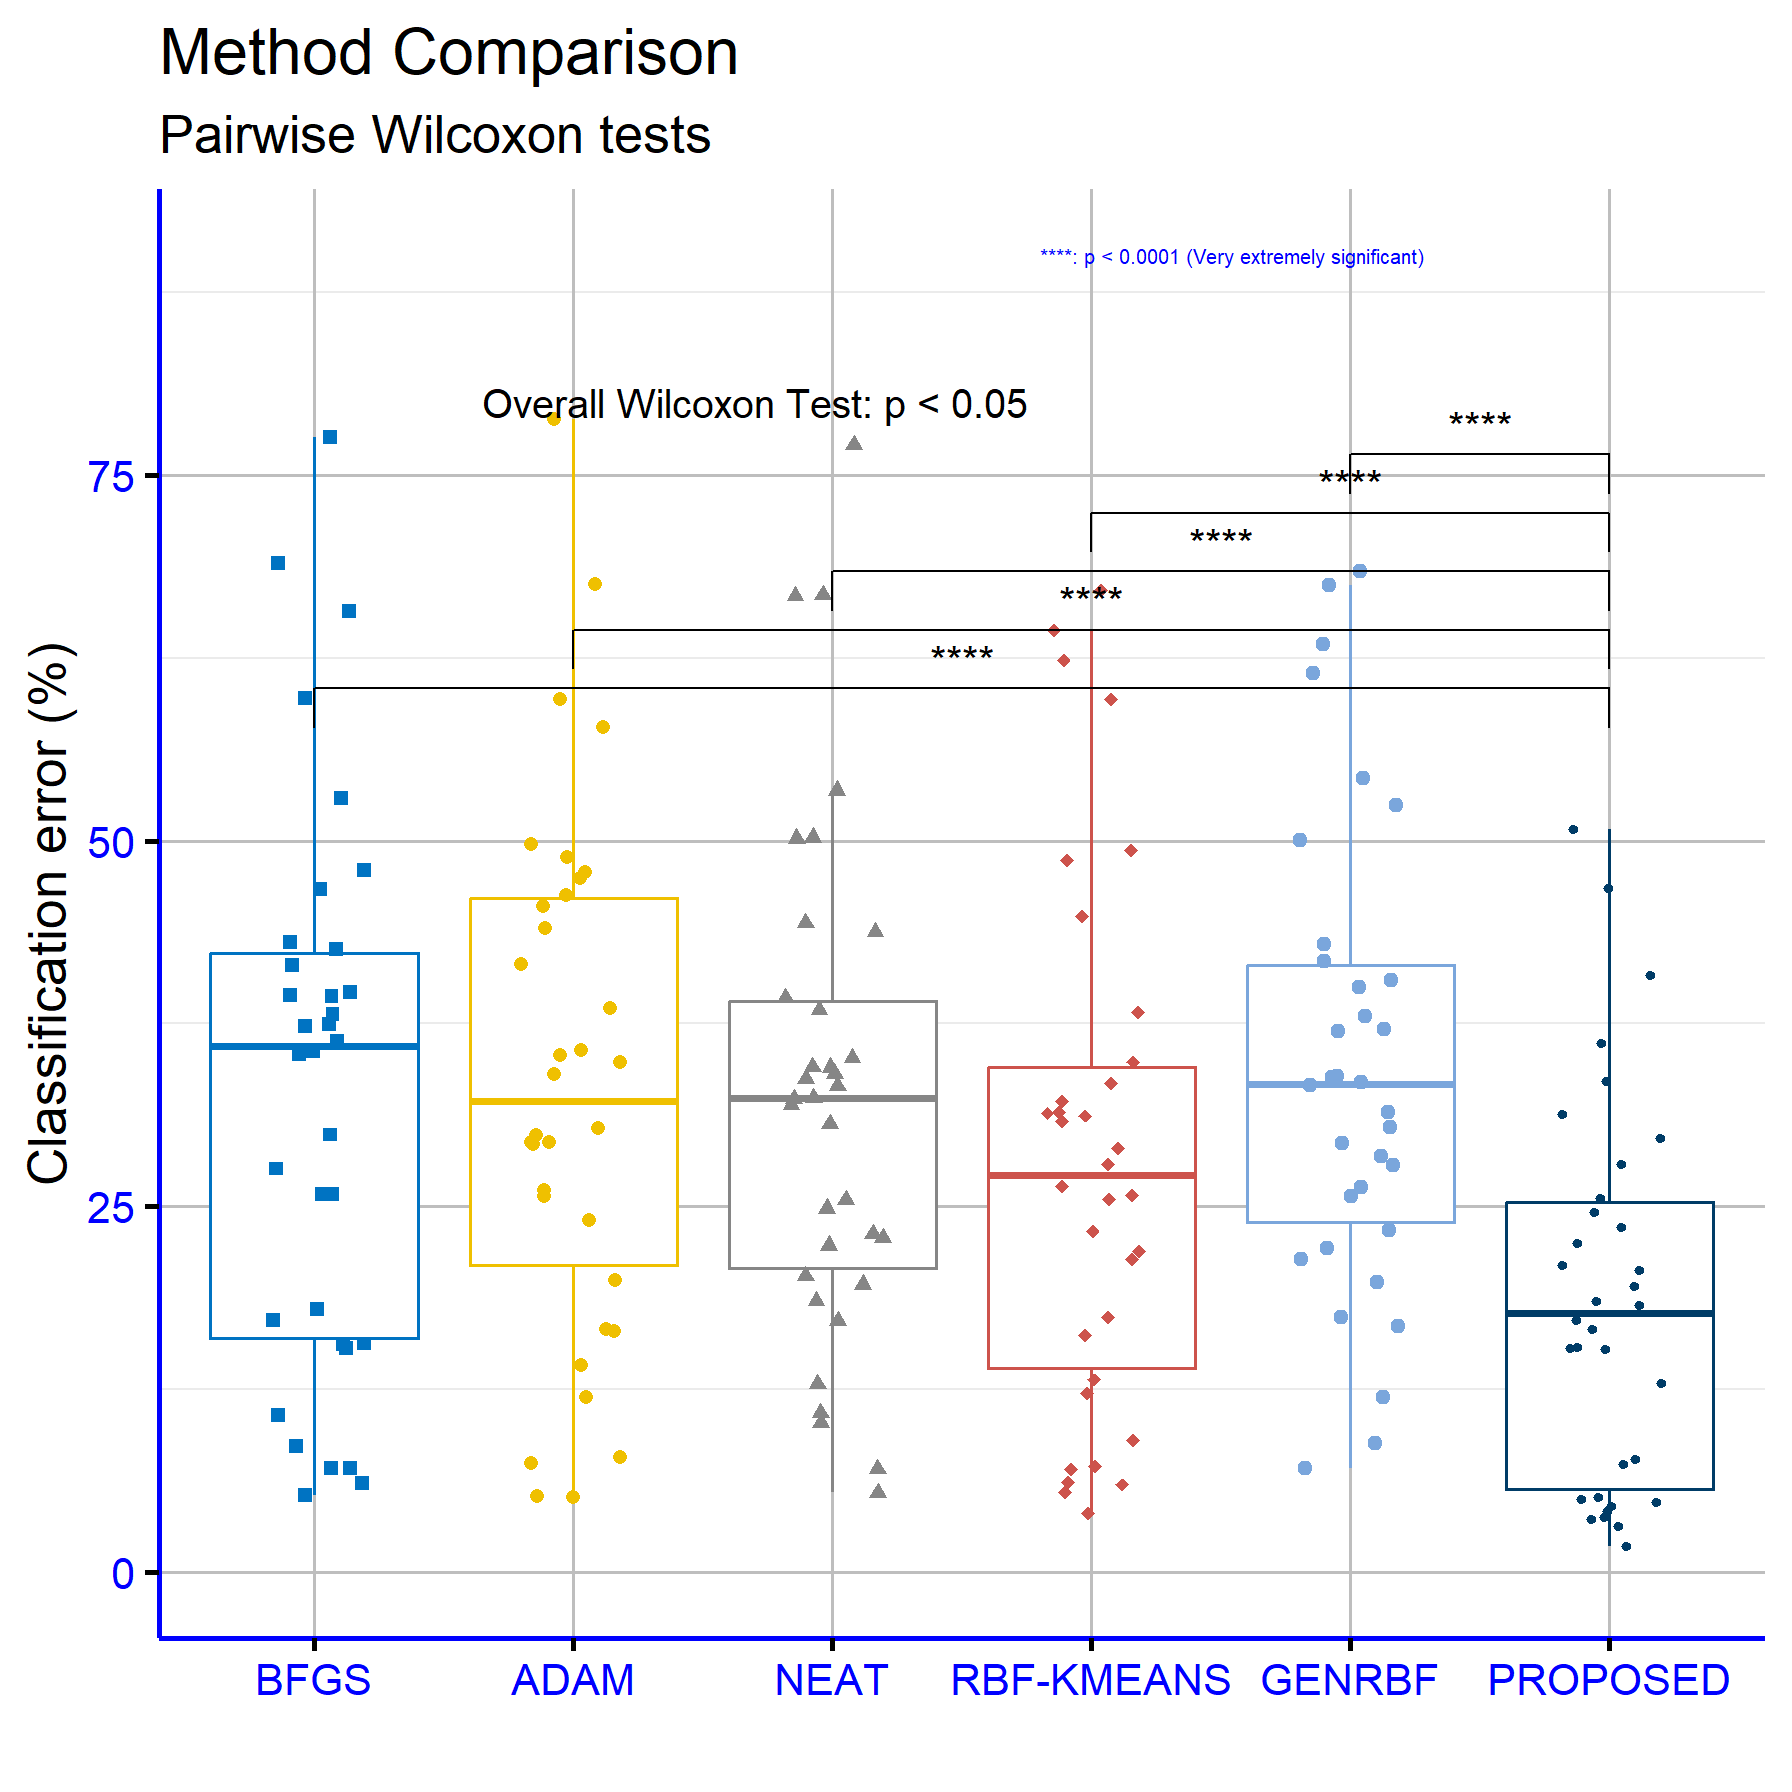
\includegraphics[scale=0.5]{img1}
\par\end{centering}
\caption{Statistical comparison of the experimental results for the classification
datasets.\protect\label{fig:statClass}}
\end{figure}
In Figure \ref{fig:statRegression}, which concerns the regression
datasets, a similar pattern is observed, though the p-values are generally
higher compared to the classification datasets. The proposed model
demonstrates statistically significant superiority over the other
models in all comparison pairs: PROPOSED vs BFGS ($p=0.00011$), PROPOSED
vs ADAM ($p=0.015$), PROPOSED vs NEAT ($p=0.00016$), PROPOSED vs
RBF-KMEANS ($p=0.0016$), and PROPOSED vs GENRBF ($p=0.00049$). Although
the significance is not as strong as in the classification datasets,
the proposed model's superiority remains clear.

\begin{figure}[H]
\begin{centering}
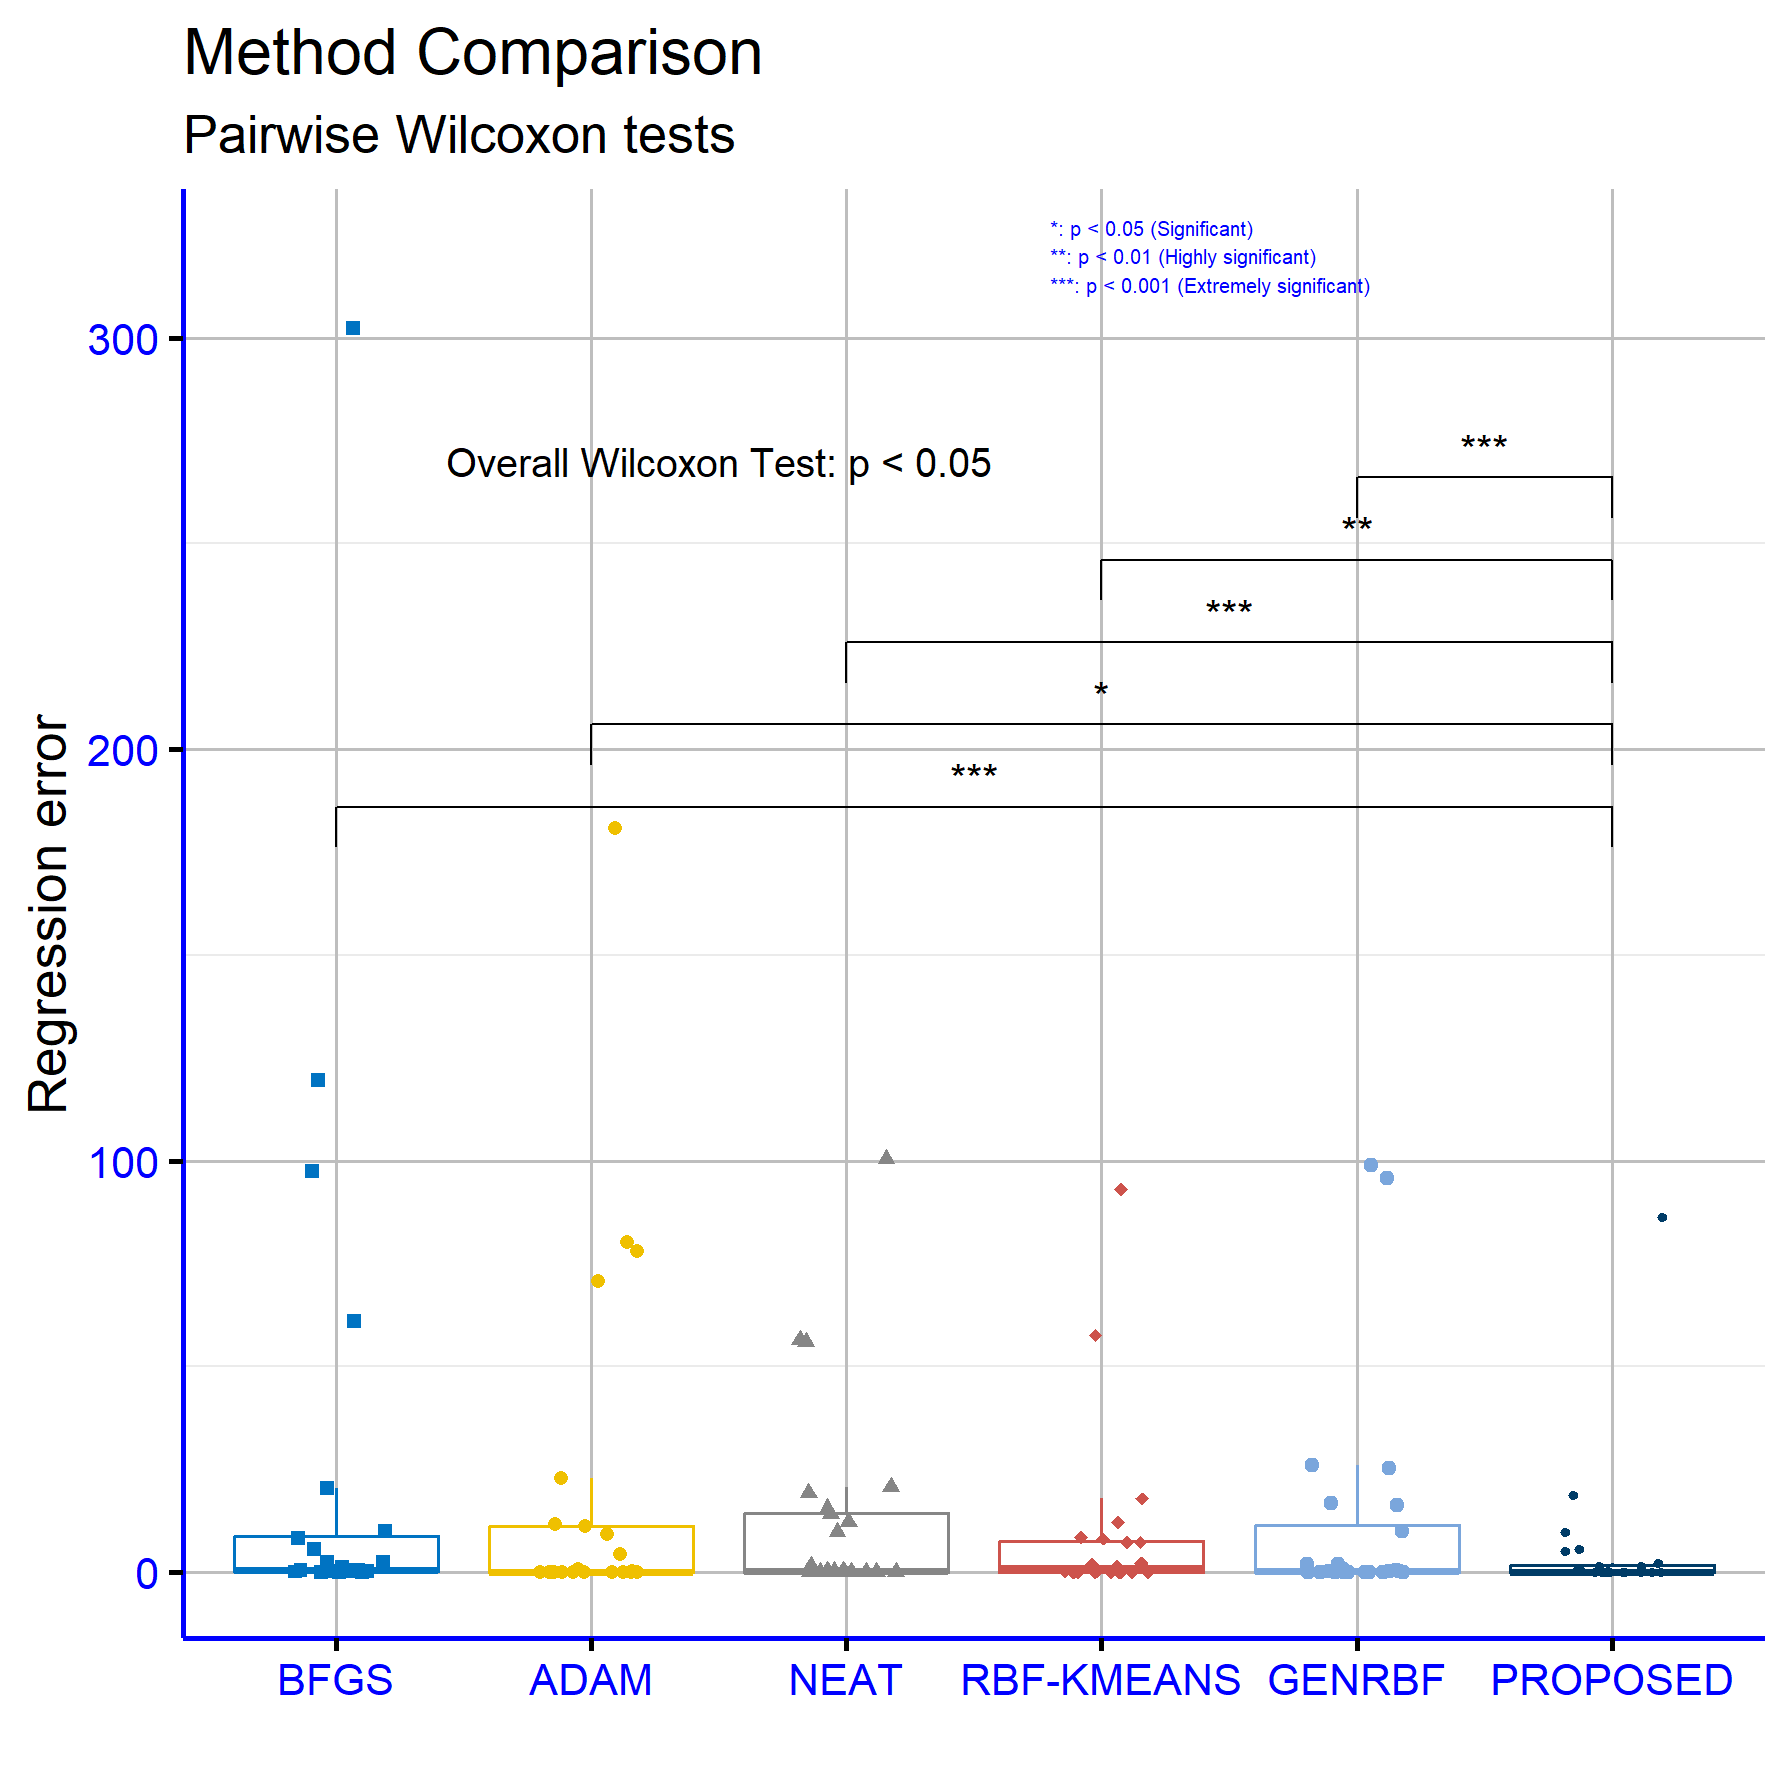
\includegraphics[scale=0.5]{img2}
\par\end{centering}
\caption{Statistical comparison of the obtained experimental results for the
regression datasets.\protect\label{fig:statRegression}}

\end{figure}


\subsection{Experiments with the perturbation factor $a$ }

In order to determine the stability of the proposed technique, another
experiment was performed in which the perturbation factor $a$ presented
in the second stage of the proposed technique took a series of different
values. The table \ref{tab:experClassA} presents the error rates
of the proposed machine learning model for three different values
of the perturbation factor $a$ (0.001, 0.005, 0.01) across various
classification datasets. Each row represents a dataset, and the values
indicate the model's error rate for each value of $a$. The last row
includes the average error rates for each value of $a$. Analysis
of the data shows that the smallest value of $a$ (0.001) achieves
the lowest average error rate (18.67\%), while the largest value (0.01)
results in the highest average (19.06\%). This suggests that the model
generally performs better with smaller values of $a$ although the
difference in averages is minimal. At the dataset level, there are
cases where the model's performance is significantly affected by changes
in the parameter. For instance, in the \textquotedbl Lymography\textquotedbl{}
dataset, increasing $a$ from 0.001 to 0.01 leads to a significant
increase in the error rate from 20.64\% to 30.33\%. A similar trend
is observed in the \textquotedbl ZOO\textquotedbl{} dataset, where
the error rate rises from 4.50\% to 6.87\% for $a=0.005$, but decreases
again to 4.60\% for $a=0.01$. On the other hand, in datasets like
\textquotedbl ZO\_NF\_S,\textquotedbl{} the error remains unchanged
at 3.63\%, regardless of changes in $a$. Datasets such as \textquotedbl Z\_F\_S\textquotedbl{}
and \textquotedbl ZONF\_S\textquotedbl{} exhibit nonlinear behavior.
In \textquotedbl Z\_F\_S,\textquotedbl{} the error rate significantly
decreases from 3.16\% to 2.79\% as $a$ increases from 0.001 to 0.01,
while in \textquotedbl ZONF\_S,\textquotedbl{} a similar decrease
is observed from 1.79\% to 1.74\%. In conclusion, the analysis indicates
that the perturbation factor $a$ has a notable impact on the performance
of the proposed model. Smaller values of $a$ are generally associated
with better performance; however, the optimal value may depend on
the characteristics of each dataset. Instances where error rates increase
or decrease nonlinearly with changes in \textquotedbl a\textquotedbl{}
suggest the need for further investigation into the tuning of \textquotedbl a\textquotedbl{}
for specific applications.

\begin{table}[H]
\caption{Experimental results for the classification datasets using a series
of values for perturbation factor $a$.\protect\label{tab:experClassA}}

\centering{}%
\begin{tabular}{|c|c|c|c|}
\hline 
\textbf{DATASET} & \textbf{$a=0.001$} & $a=0.005$ & $a=0.01$\tabularnewline
\hline 
\hline 
Alcohol & 31.28\% & 30.88\% & 31.77\%\tabularnewline
\hline 
Appendicitis & 15.27\% & 15.77\% & 15.57\%\tabularnewline
\hline 
Australian & 21.00\% & 21.03\% & 20.77\%\tabularnewline
\hline 
Balance & 12.95\% & 13.13\% & 13.29\%\tabularnewline
\hline 
Cleveland & 50.82\% & 50.64\% & 51.11\%\tabularnewline
\hline 
Circular & 4.19\% & 4.01\% & 4.08\%\tabularnewline
\hline 
Dermatology & 36.13\% & 36.81\% & 36.67\%\tabularnewline
\hline 
Hayes Roth & 33.54\% & 33.44\% & 34.10\%\tabularnewline
\hline 
Heart & 15.33\% & 15.15\% & 15.22\%\tabularnewline
\hline 
HeartAttack & 18.52\% & 18.80\% & 18.88\%\tabularnewline
\hline 
HouseVotes & 3.74\% & 3.60\% & 4.12\%\tabularnewline
\hline 
Ionosphere & 7.39\% & 7.38\% & 7.29\%\tabularnewline
\hline 
Liverdisorder & 27.92\% & 28.27\% & 28.49\%\tabularnewline
\hline 
Lymography & 20.64\% & 20.57\% & 30.33\%\tabularnewline
\hline 
Mammographic & 17.21\% & 17.15\% & 17.14\%\tabularnewline
\hline 
Parkinsons & 15.35\% & 14.35\% & 15.23\%\tabularnewline
\hline 
Phoneme & 16.62\% & 16.74\% & 16.00\%\tabularnewline
\hline 
Pima & 23.59\% & 24.09\% & 23.99\%\tabularnewline
\hline 
Popfailures & 4.80\% & 4.82\% & 4.86\%\tabularnewline
\hline 
Regions2 & 25.54\% & 25.62\% & 25.75\%\tabularnewline
\hline 
Saheart & 29.64\% & 29.93\% & 29.22\%\tabularnewline
\hline 
Segment & 40.83\% & 41.41\% & 41.96\%\tabularnewline
\hline 
Sonar & 18.25\% & 17.80\% & 17.83\%\tabularnewline
\hline 
Spiral & 22.52\% & 22.00\% & 22.27\%\tabularnewline
\hline 
Statheart & 19.52\% & 19.35\% & 19.58\%\tabularnewline
\hline 
Student & 5.11\% & 5.03\% & 5.25\%\tabularnewline
\hline 
Transfusion & 24.59\% & 24.70\% & 24.64\%\tabularnewline
\hline 
Wdbc & 5.00\% & 5.05\% & 5.07\%\tabularnewline
\hline 
Wine & 7.71\% & 7.88\% & 7.90\%\tabularnewline
\hline 
Z\_F\_S & 3.16\% & 3.66\% & 2.79\%\tabularnewline
\hline 
Z\_O\_N\_F\_S & 46.77\% & 46.83\% & 47.06\%\tabularnewline
\hline 
ZO\_NF\_S & 3.63\% & 3.63\% & 3.63\%\tabularnewline
\hline 
ZONF\_S & 1.79\% & 1.81\% & 1.74\%\tabularnewline
\hline 
ZOO & 4.50\% & 6.87\% & 4.60\%\tabularnewline
\hline 
\textbf{AVERAGE} & \textbf{18.67\%} & \textbf{18.77\%} & \textbf{19.06\%}\tabularnewline
\hline 
\end{tabular}
\end{table}
The table \ref{tab:experRegressionA} displays the absolute error
values of the proposed machine learning model across various regression
datasets for three different values of the perturbation factor $a$
(0.001, 0.005, 0.01). Data analysis reveals that the parameter $a=0.005$
yields the lowest average error (4.92), while the values $a=0.001$
and $a=0.01$ result in slightly higher averages (5.48 and 5.13, respectively).
This difference indicates that 0.005 is generally the most suitable
value for the model, ensuring better performance in most cases. At
the dataset level, the impact of $a$ varies. Some datasets, such
as \textquotedbl Airfoil,\textquotedbl{} \textquotedbl Concrete,\textquotedbl{}
\textquotedbl Dee,\textquotedbl{} \textquotedbl HO,\textquotedbl{}
\textquotedbl Laser,\textquotedbl{} \textquotedbl NT,\textquotedbl{}
\textquotedbl PL,\textquotedbl{} \textquotedbl Plastic,\textquotedbl{}
and \textquotedbl Quake,\textquotedbl{} show no change in error with
variations in $a$ as error values remain constant. In contrast, other
datasets exhibit significant variations. For example, in the \textquotedbl Baseball\textquotedbl{}
dataset, the error decreases from 86.19 for $a=0.001$ to 77.46 for
$a=0.005$ then increases again to 81.97 for $a=0.01$. Similarly,
in the \textquotedbl MB\textquotedbl{} dataset, the error drastically
decreases from 5.49 for $a=0.001$ to 0.56 for $a=0.005$ and further
to 0.48 for $a=0.01$. In datasets like \textquotedbl FA\textquotedbl{}
and \textquotedbl FY,\textquotedbl{} the error increases as $a$
changes from 0.001 to 0.005, then decreases again for $a=0.01$. In
the \textquotedbl Treasury\textquotedbl{} dataset, the error shows
a slight decline as $a$ increases. In conclusion, the parameter $a$
has a significant impact on the model's performance in certain datasets,
while in others, its effect is negligible. The lowest average error
observed for $a=0.005$ suggests that this value is generally optimal
for the model, though further tuning may be required for specific
datasets. Cases with high variability in errors highlight the need
for deeper analysis and optimization of the $a$ parameter based on
the characteristics of each dataset.

\begin{table}[H]
\caption{Experimental results for regression datasets using different values
for parameter $a$.\protect\label{tab:experRegressionA}}

\centering{}%
\begin{tabular}{|c|c|c|c|}
\hline 
\textbf{DATASET} & $a=0.001$ & $a=0.005$ & $a=0.01$\tabularnewline
\hline 
Abalone & 5.10 & 5.12 & 5.10\tabularnewline
\hline 
Airfoil & 0.004 & 0.004 & 0.004\tabularnewline
\hline 
Auto & 9.68 & 9.80 & 9.89\tabularnewline
\hline 
Baseball & 86.19 & 77.46 & 81.97\tabularnewline
\hline 
BK & 0.153 & 0.043 & 0.11\tabularnewline
\hline 
BL & 0.0002 & 0.0002 & 0.0003\tabularnewline
\hline 
Concrete & 0.006 & 0.006 & 0.006\tabularnewline
\hline 
Dee & 0.16 & 0.16 & 0.16\tabularnewline
\hline 
Housing & 18.70 & 18.73 & 19.20\tabularnewline
\hline 
Friedman & 1.45 & 1.44 & 1.45\tabularnewline
\hline 
FA & 0.019 & 0.09 & 0.07\tabularnewline
\hline 
FY & 0.077 & 0.12 & 0.076\tabularnewline
\hline 
HO & 0.01 & 0.01 & 0.01\tabularnewline
\hline 
Laser & 0.003 & 0.003 & 0.003\tabularnewline
\hline 
MB & 5.49 & 0.56 & 0.48\tabularnewline
\hline 
Mortgage & 0.14 & 0.12 & 0.13\tabularnewline
\hline 
NT & 0.007 & 0.007 & 0.007\tabularnewline
\hline 
PL & 0.023 & 0.023 & 0.023\tabularnewline
\hline 
Plastic & 2.29 & 2.29 & 2.29\tabularnewline
\hline 
PY & 0.019 & 0.019 & 0.017\tabularnewline
\hline 
Quake & 0.036 & 0.036 & 0.036\tabularnewline
\hline 
SN & 0.024 & 0.025 & 0.024\tabularnewline
\hline 
Stock & 1.53 & 1.52 & 1.52\tabularnewline
\hline 
Treasury & 0.51 & 0.54 & 0.47\tabularnewline
\hline 
\textbf{AVERAGE} & \textbf{5.48} & \textbf{4.92} & \textbf{5.13}\tabularnewline
\hline 
\end{tabular}
\end{table}
Figure \ref{fig:statClassA} compares different values of parameter
$a$ for the classification datasets. The p-values for the comparisons
$a=0.001$ vs $a=0.005$ ($p=0.36$), $a=0.001$ vs $a=0.01$ ($p=0.071$),
and $a=0.005$ vs $a=0.01$ ($p=0.17$) indicate that the differences
between the parameter values are not statistically significant. This
suggests that varying parameter $a$ within this range does not substantially
affect the model's performance on these datasets.

\begin{figure}[H]
\begin{centering}
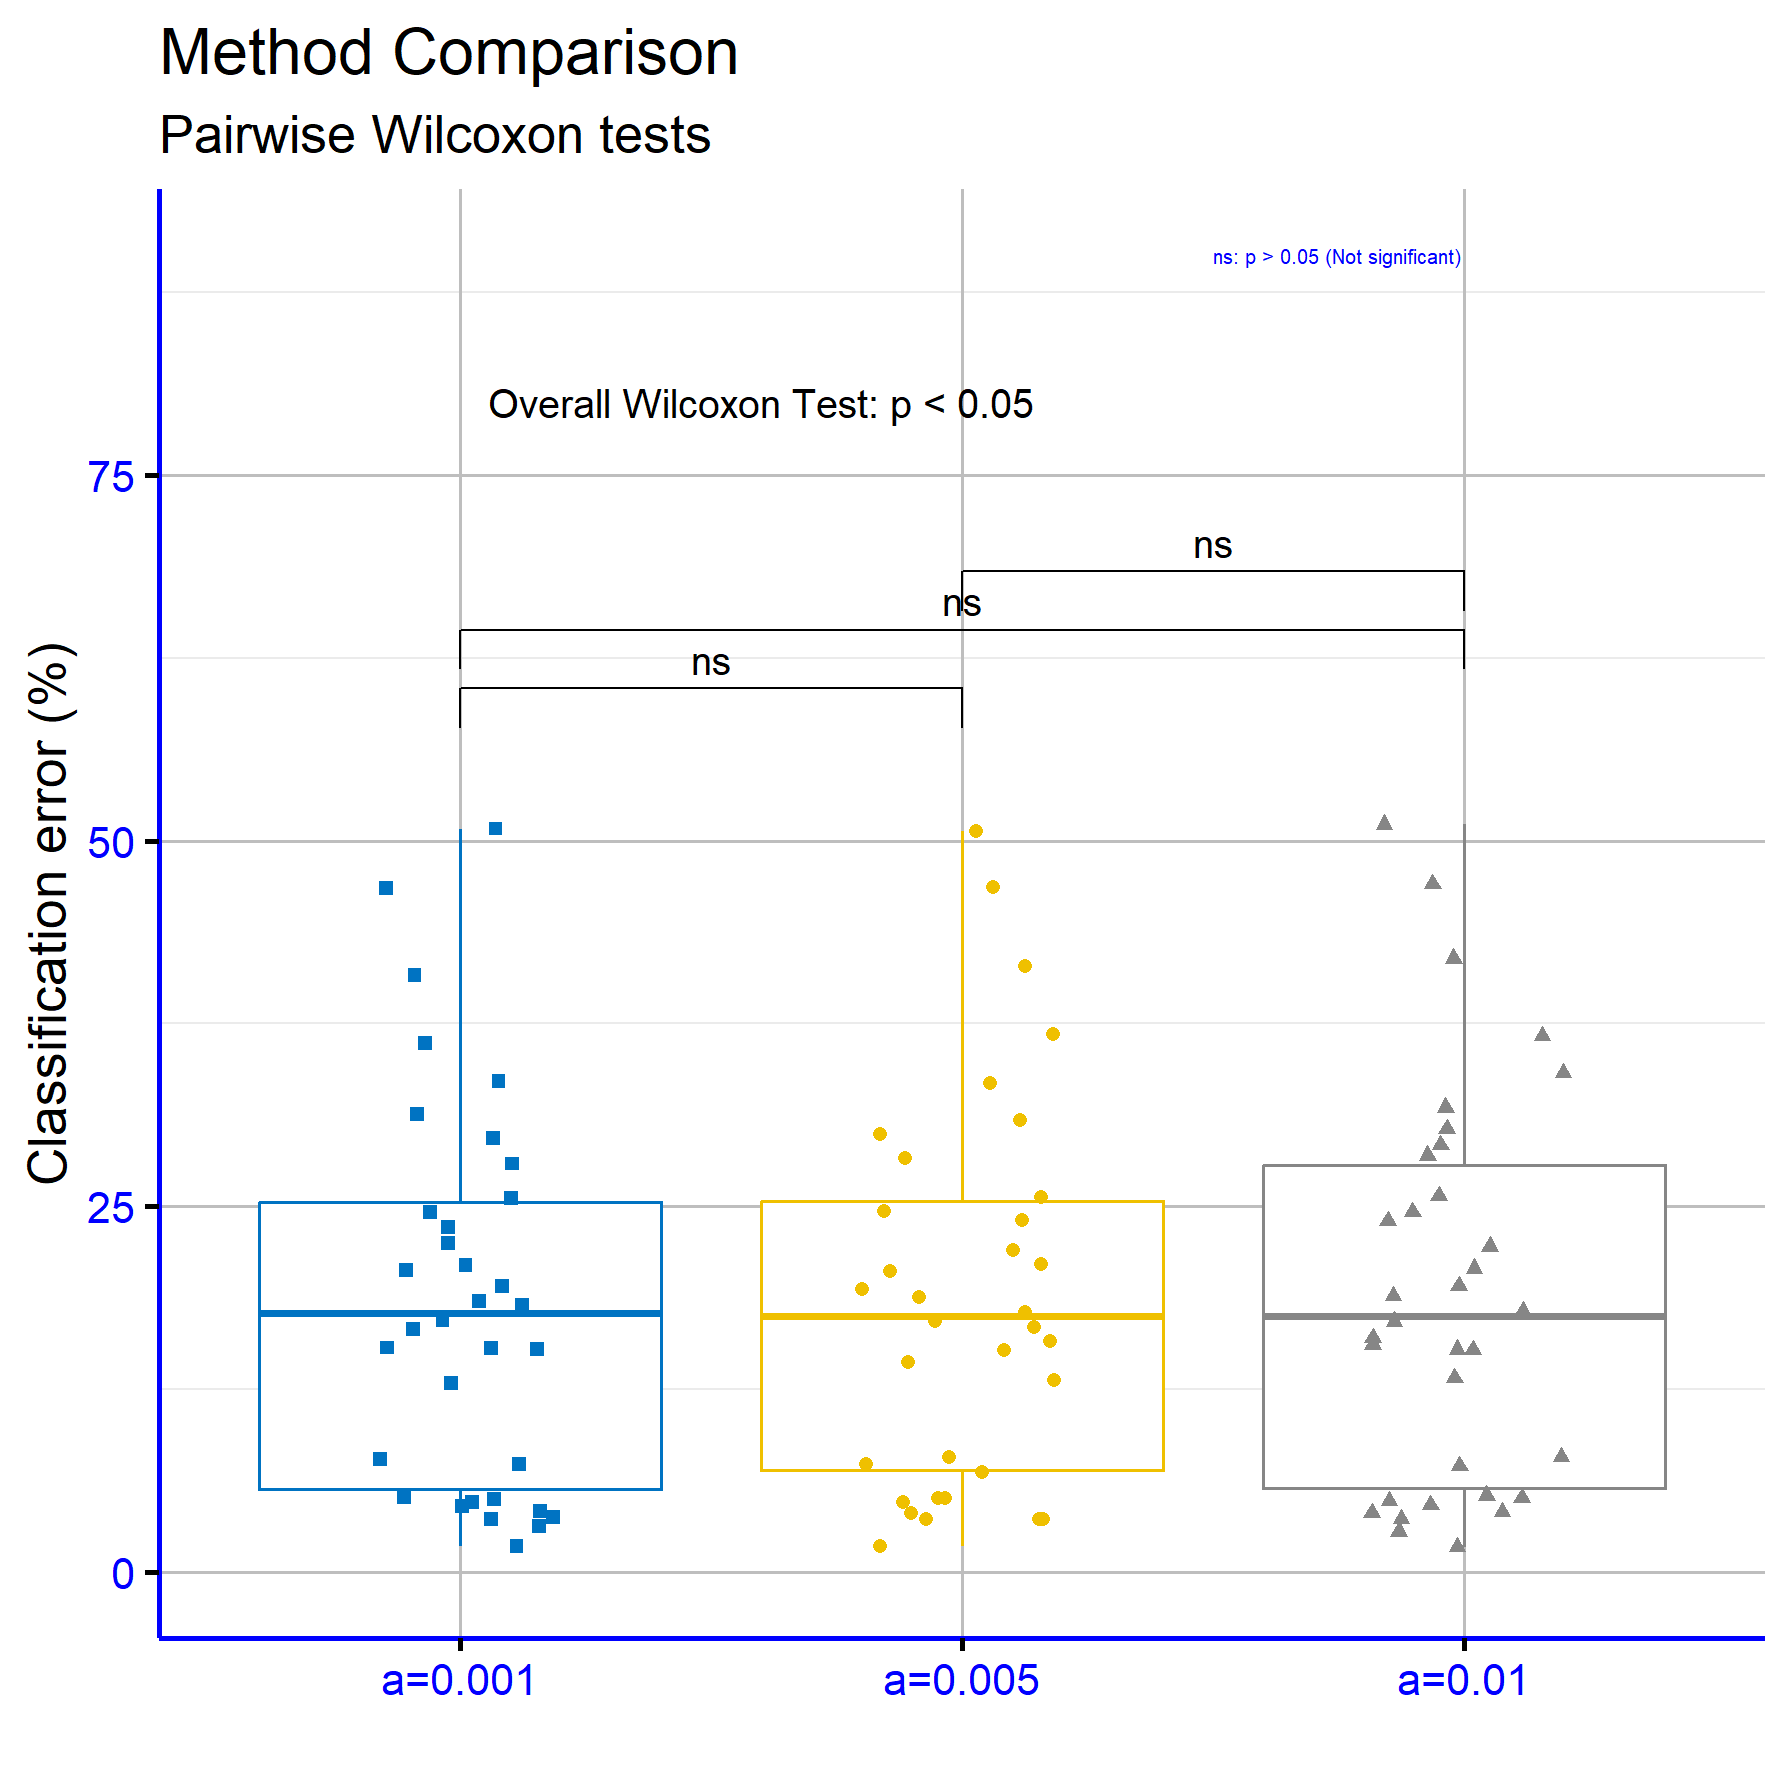
\includegraphics[scale=0.5]{img3}
\par\end{centering}
\caption{Statistical comparison of the obtained results from the application
of the current method in the classification datasets using different
values of perturbation factor $a$.\protect\label{fig:statClassA}}

\end{figure}
Figure \ref{fig:statRegressionA} presents corresponding comparisons
for the regression datasets, where a similar result is observed. The
p-values for the comparisons $a=0.001$ vs $a=0.005$ ($p=0.75$),
$a=0.001$ vs $a=0.01$ ($p=0.41$), and $a=0.005$ vs $a=0.01$ ($p=0.94$)
indicate the absence of statistically significant differences. This
shows that the choice of parameter $a$ does not significantly influence
the model's performance on the regression datasets.
\begin{figure}[H]
\begin{centering}
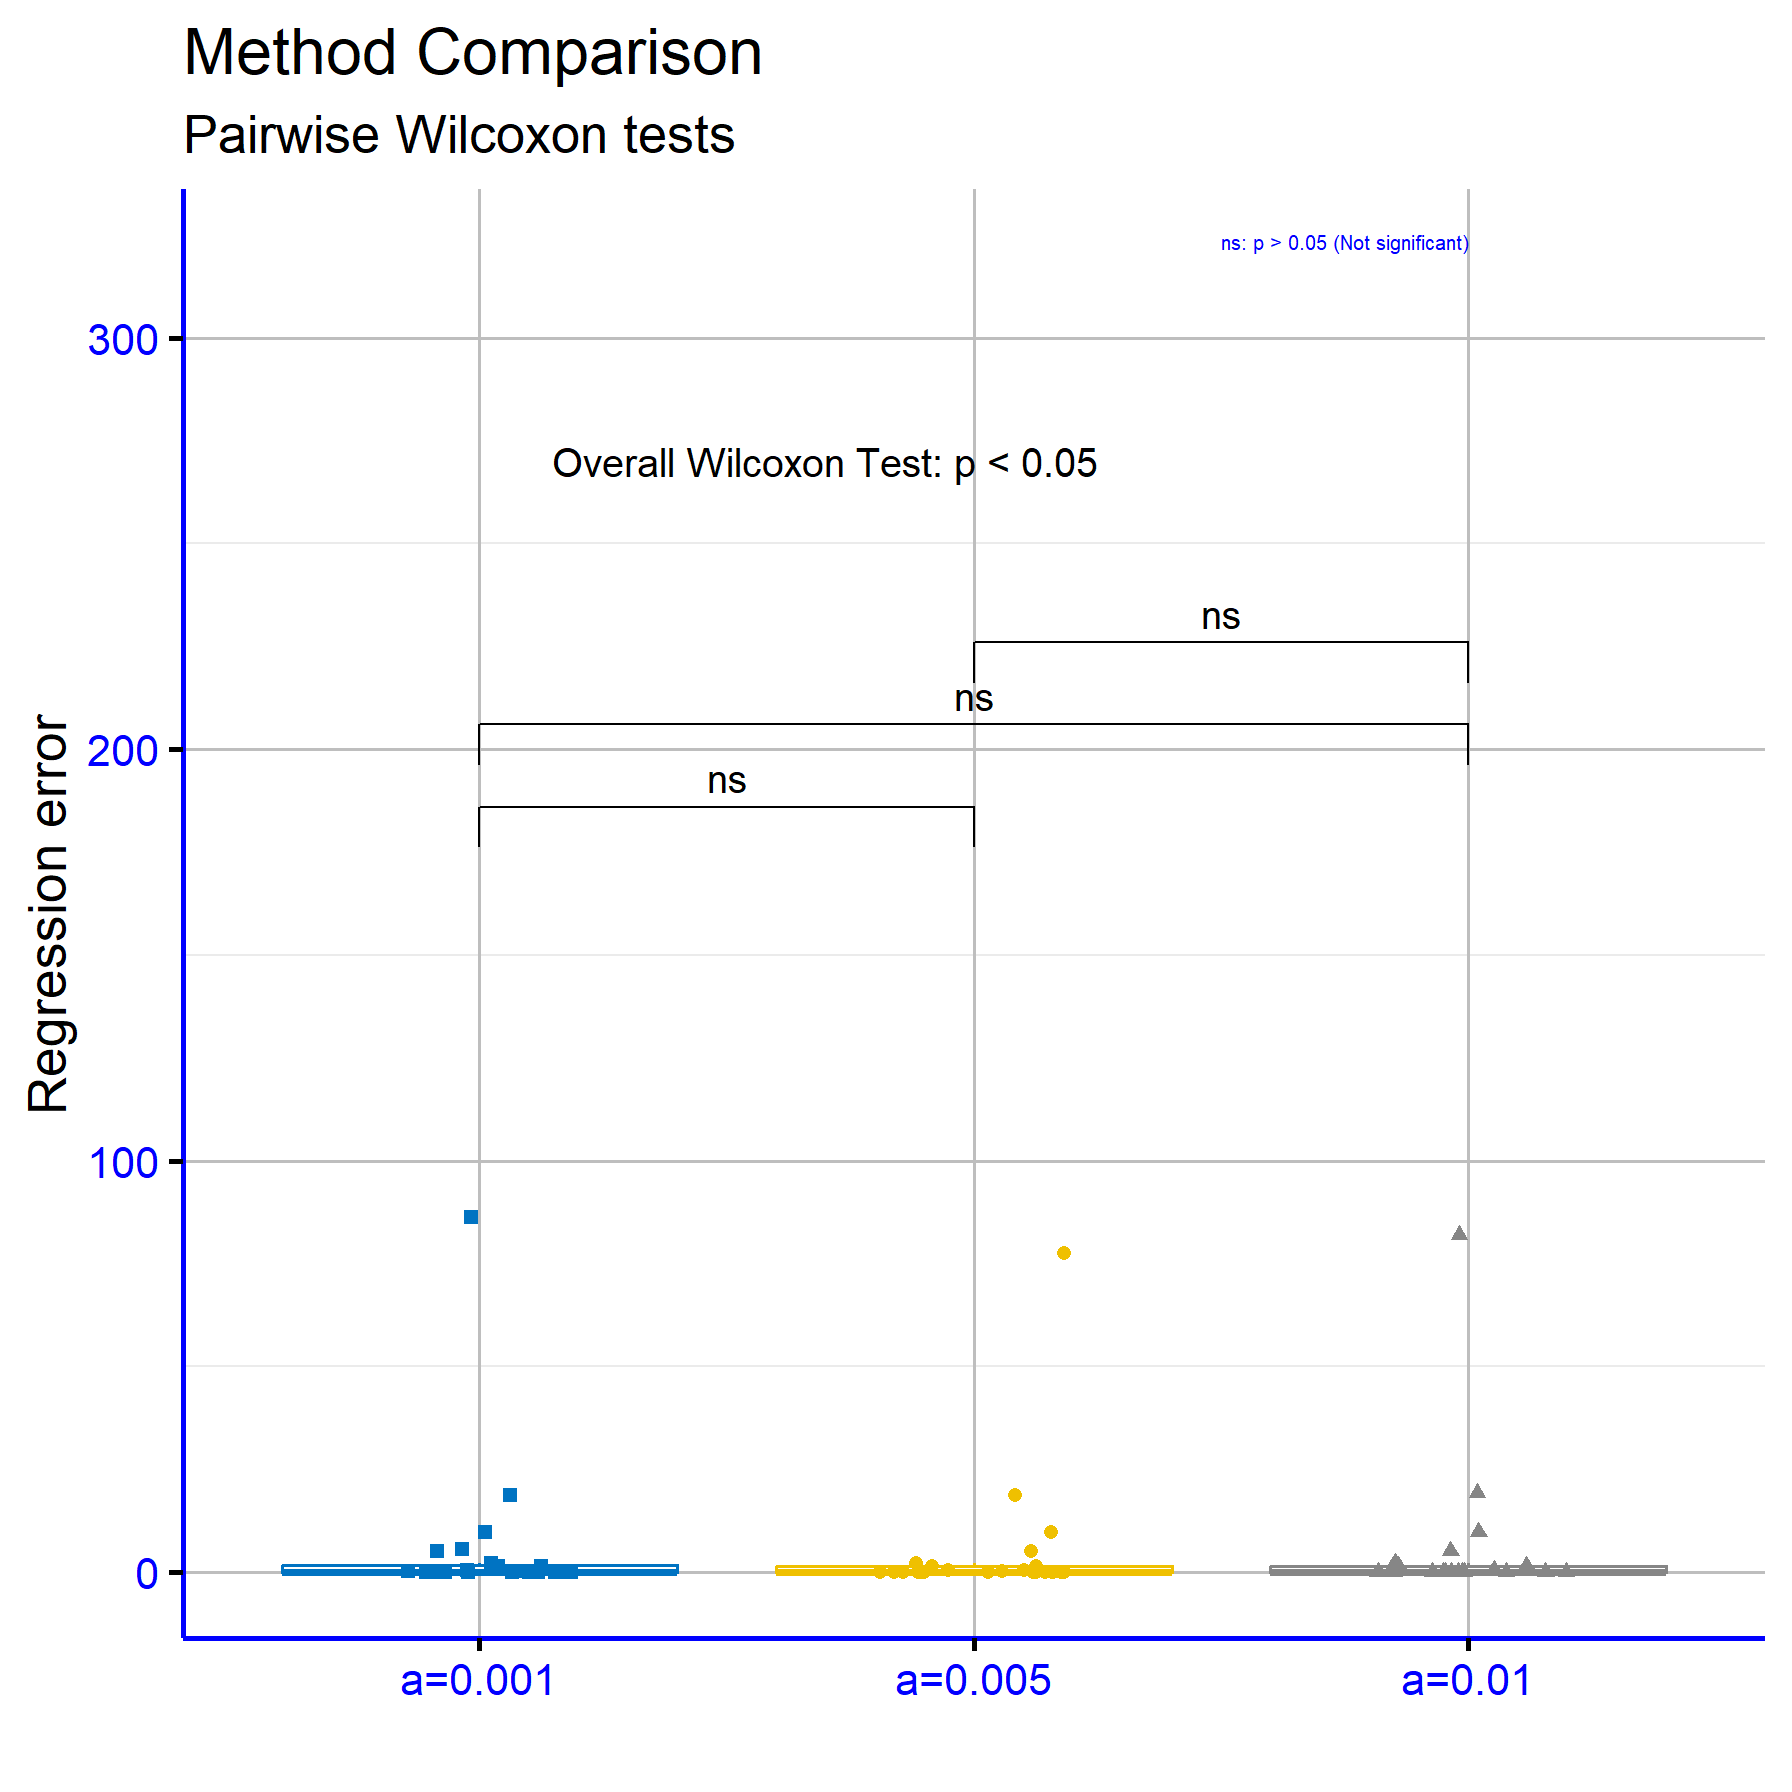
\includegraphics[scale=0.5]{img4}
\par\end{centering}
\caption{Statistical comparison of the obtained experiments results from the
application of the proposed method to the regression datasets, using
different values of the perturbation factor $a$.\protect\label{fig:statRegressionA}}

\end{figure}


\subsection{Experiments with the parameter $F$}

Another experiment was conducted using the initialization factor $F$.
Table \ref{tab:experClassF} presents the percentage error rates of
the proposed machine learning model across various classification
datasets for four different values of the parameter $F$ (1.5, 3.0,
5.0, 10.0). Analyzing the data reveals that the parameter $F$ influences
the model's performance, but this effect varies by dataset. The lowest
average error rate is observed for $F=5.0$ (18.58\%), indicating
that this value is generally optimal. For the other values, slightly
higher average error rates are noted: 18.88\% for $F=3.0$ 18.67\%
for $F=10.0$ and the highest rate, 20.32\%, for $F=1.5$. Examining
individual datasets, it is evident that for many of them, increasing
$F$ improves performance, as reflected in reduced error rates. Examples
include the \textquotedbl Ionosphere,\textquotedbl{} \textquotedbl Wine,\textquotedbl{}
and \textquotedbl ZONF\_S\textquotedbl{} datasets, where error rates
decrease as $F$ increases. In \textquotedbl Ionosphere,\textquotedbl{}
the error rate drops from 12.92\% for $F=1.5$ to 7.39\% for $F=10.0$.
In \textquotedbl Wine,\textquotedbl{} the error rate decreases from
10.90\% for $F=1.5$ to 7.71\% for $F=10.0$. Similarly, in \textquotedbl ZONF\_S,\textquotedbl{}
the error rate steadily decreases from 2.59\% for $F=1.5$ to 1.79\%
for $F=10.0$. However, there are cases where increasing $F$ does
not lead to improvement or results in higher error rates. For example,
in the \textquotedbl Segment\textquotedbl{} dataset, the error rate
rises from 35.81\% for $F=1.5$ to 40.83\% for $F=10.0$. In the \textquotedbl Spiral\textquotedbl{}
dataset, the error rate consistently increases from 13.28\% for $F=1.5$
to 22.52\% for $F=10.0$. A similar trend is observed in the \textquotedbl Z\_O\_N\_F\_S\textquotedbl{}
dataset, where the error rate rises from 46.00\% for $F=1.5$ to 46.77\%
for $F=10.0$. Overall, the parameter $F$ significantly affects the
model's performance, and the optimal value appears to be $F=5.0$
as evidenced by the lowest average error rate. However, the exact
impact depends on the characteristics of each dataset, emphasizing
the need to fine-tune the parameter value for specific datasets to
achieve optimal performance.

\begin{table}[H]
\caption{Experimental results for the classification datasets using a series
of values for parameter $F$.\protect\label{tab:experClassF}}

\centering{}%
\begin{tabular}{|c|c|c|c|c|}
\hline 
\textbf{DATASET} & $F=1.5$ & $F=3.0$ & $F=5.0$ & \textbf{$F=10.0$}\tabularnewline
\hline 
\hline 
Alcohol & 25.66\% & 29.16\% & 26.14\% & 31.28\%\tabularnewline
\hline 
Appendicitis & 16.30\% & 14.57\% & 15.50\% & 15.27\%\tabularnewline
\hline 
Australian & 23.53\% & 22.27\% & 20.81\% & 21.00\%\tabularnewline
\hline 
Balance & 15.12\% & 13.32\% & 12.68\% & 12.95\%\tabularnewline
\hline 
Cleveland & 51.81\% & 51.41\% & 50.70\% & 50.82\%\tabularnewline
\hline 
Circular & 4.75\% & 4.15\% & 4.52\% & 4.19\%\tabularnewline
\hline 
Dermatology & 36.69\% & 36.48\% & 36.39\% & 36.13\%\tabularnewline
\hline 
Hayes Roth & 46.18\% & 35.54\% & 34.18\% & 33.54\%\tabularnewline
\hline 
Heart & 16.68\% & 15.93\% & 15.68\% & 15.33\%\tabularnewline
\hline 
HeartAttack & 27.39\% & 20.38\% & 19.03\% & 18.52\%\tabularnewline
\hline 
HouseVotes & 3.80\% & 3.35\% & 3.85\% & 3.74\%\tabularnewline
\hline 
Ionosphere & 12.92\% & 8.27\% & 7.41\% & 7.39\%\tabularnewline
\hline 
Liverdisorder & 30.48\% & 29.27\% & 28.48\% & 27.92\%\tabularnewline
\hline 
Lymography & 29.89\% & 22.41\% & 21.93\% & 20.64\%\tabularnewline
\hline 
Mammographic & 18.00\% & 17.17\% & 16.96\% & 17.21\%\tabularnewline
\hline 
Parkinsons & 18.25\% & 17.18\% & 15.90\% & 15.35\%\tabularnewline
\hline 
Phoneme & 17.27\% & 15.88\% & 15.90\% & 16.62\%\tabularnewline
\hline 
Pima & 24.54\% & 24.17\% & 24.05\% & 23.59\%\tabularnewline
\hline 
Popfailures & 7.07\% & 5.35\% & 5.01\% & 4.80\%\tabularnewline
\hline 
Regions2 & 26.07\% & 26.02\% & 25.78\% & 25.54\%\tabularnewline
\hline 
Saheart & 29.75\% & 28.91\% & 29.42\% & 29.64\%\tabularnewline
\hline 
Segment & 35.81\% & 36.84\% & 38.93\% & 40.83\%\tabularnewline
\hline 
Sonar & 24.68\% & 19.25\% & 16.98\% & 18.25\%\tabularnewline
\hline 
Spiral & 13.28\% & 15.25\% & 17.88\% & 22.52\%\tabularnewline
\hline 
Statheart & 19.98\% & 19.58\% & 19.63\% & 19.52\%\tabularnewline
\hline 
Student & 6.14\% & 6.30\% & 5.92\% & 5.11\%\tabularnewline
\hline 
Transfusion & 25.45\% & 25.23\% & 25.19\% & 24.59\%\tabularnewline
\hline 
Wdbc & 4.94\% & 4.92\% & 4.90\% & 5.00\%\tabularnewline
\hline 
Wine & 10.90\% & 9.37\% & 8.51\% & 7.71\%\tabularnewline
\hline 
Z\_F\_S & 4.13\% & 3.73\% & 3.67\% & 3.16\%\tabularnewline
\hline 
Z\_O\_N\_F\_S & 46.00\% & 45.61\% & 46.57\% & 46.77\%\tabularnewline
\hline 
ZO\_NF\_S & 3.67\% & 4.19\% & 3.16\% & 3.63\%\tabularnewline
\hline 
ZONF\_S & 2.59\% & 2.37\% & 2.06\% & 1.79\%\tabularnewline
\hline 
ZOO & 11.17\% & 8.10\% & 8.00\% & 4.50\%\tabularnewline
\hline 
\textbf{AVERAGE} & \textbf{20.32\%} & \textbf{18.88\%} & \textbf{18.58\%} & \textbf{18.67\%}\tabularnewline
\hline 
\end{tabular}
\end{table}
Table \ref{tab:experRegressionF} provides the absolute error values
of the proposed machine learning model across various regression datasets
for four different values of the parameter $F$ (1.5, 3.0, 5.0, 10.0).
The data analysis shows that the parameter $F$ affects the model's
performance differently depending on the dataset. The average errors
indicate that $F=5.0$ yields the lowest overall error (5.22), followed
by $F=3.0$ with an average of 5.25. Higher averages are observed
for $F=1.5$ (5.52) and $F=10.0$ (5.48), suggesting that deviating
from $F=5.0$ tends to increase error in some cases. Examining the
datasets, it is evident that in several cases, increasing $F$ improves
performance, reducing error rates. For example, in the \textquotedbl Abalone\textquotedbl{}
dataset, the error decreases from 6.39 for $F=1.5$ to 5.10 for $F=10.0$.
Similarly, in the \textquotedbl Friedman\textquotedbl{} dataset,
the error significantly decreases from 6.59 for $F=1.5$ to 1.45 for
$F=10.0$. In the \textquotedbl Laser\textquotedbl{} dataset, the
error decreases progressively from 0.022 for $F=1.5$ to 0.003 for
$F=10.0$. Conversely, there are datasets where the effect of $F$
is nonlinear or increases the error rate. For instance, in the \textquotedbl Housing\textquotedbl{}
dataset, the error rises from 16.75 for $F=1.5$ to 18.70 for $F=10.0$.
In the \textquotedbl MB\textquotedbl{} dataset, there is a sharp
increase in error from 0.116 for $F=1.5$ to 5.49 for $F=10.0$, indicating
that $F$ significantly impacts model performance for this dataset.
In summary, the parameter $F$ has varying effects on the model's
performance across different datasets. While the average indicates
that $F=5.0$ is the optimal choice, precise optimization of the parameter
should be dataset-specific. Additionally, extreme parameter values
may lead to significant performance degradation in certain datasets,
as seen in examples like \textquotedbl MB\textquotedbl{} and \textquotedbl Housing.\textquotedbl{}

\begin{table}[H]
\caption{Experimental results for regression datasets using different values
for parameter $F$.\protect\label{tab:experRegressionF}}

\centering{}%
\begin{tabular}{|c|c|c|c|c|}
\hline 
\textbf{DATASET} & $F=1.5$ & $F=3.0$ & $F=5.0$ & $F=10.0$\tabularnewline
\hline 
Abalone & 6.39 & 5.79 & 5.57 & 5.10\tabularnewline
\hline 
Airfoil & 0.004 & 0.004 & 0.004 & 0.004\tabularnewline
\hline 
Auto & 9.83 & 9.69 & 9.67 & 9.68\tabularnewline
\hline 
Baseball & 84.27 & 83.01 & 84.57 & 86.19\tabularnewline
\hline 
BK & 0.275 & 0.048 & 0.071 & 0.153\tabularnewline
\hline 
BL & 0.41 & 0.0005 & 0.0003 & 0.0002\tabularnewline
\hline 
Concrete & 0.006 & 0.006 & 0.006 & 0.006\tabularnewline
\hline 
Dee & 0.16 & 0.16 & 0.16 & 0.16\tabularnewline
\hline 
Housing & 16.75 & 17.82 & 18.07 & 18.70\tabularnewline
\hline 
Friedman & 6.59 & 3.85 & 1.67 & 1.45\tabularnewline
\hline 
FA & 0.054 & 0.03 & 0.053 & 0.019\tabularnewline
\hline 
FY & 0.216 & 0.246 & 0.332 & 0.077\tabularnewline
\hline 
HO & 0.01 & 0.01 & 0.01 & 0.01\tabularnewline
\hline 
Laser & 0.022 & 0.011 & 0.005 & 0.003\tabularnewline
\hline 
MB & 0.116 & 0.135 & 0.307 & 5.49\tabularnewline
\hline 
Mortgage & 0.56 & 0.59 & 0.36 & 0.14\tabularnewline
\hline 
NT & 0.007 & 0.007 & 0.007 & 0.007\tabularnewline
\hline 
PL & 0.024 & 0.023 & 0.023 & 0.023\tabularnewline
\hline 
Plastic & 2.37 & 2.33 & 2.31 & 2.29\tabularnewline
\hline 
PY & 2.33 & 0.049 & 0.022 & 0.019\tabularnewline
\hline 
Quake & 0.036 & 0.036 & 0.036 & 0.036\tabularnewline
\hline 
SN & 0.028 & 0.04 & 0.025 & 0.024\tabularnewline
\hline 
Stock & 1.45 & 1.51 & 1.49 & 1.53\tabularnewline
\hline 
Treasury & 0.50 & 0.59 & 0.43 & 0.51\tabularnewline
\hline 
\textbf{AVERAGE} & \textbf{5.52} & \textbf{5.25} & \textbf{5.22} & \textbf{5.48}\tabularnewline
\hline 
\end{tabular}
\end{table}
In Figure \ref{fig:statClassF}, which compares different values of
parameter $F$ for the classification datasets, several statistically
significant differences are observed. The p-values for the comparisons
$F=1.5$ vs $F=3.0$ ($p=0.00019$), $F=1.5$ vs $F=5.0$ ($p=0.00012$),
and $F=1.5$ vs $F=10.0$ ($p=0.00069$) indicate a strong difference
in the model's performance. In contrast, the values for the comparisons
$F=3.0$ vs $F=5.0$ ($p=0.027$), $F=3.0$ vs $F=10.0$ ($p=0.062$),
and $F=5.0$ vs $F=10.0$ ($p=0.23$) show that the differences between
larger values of parameter $F$ are less significant.

\begin{figure}[H]
\begin{centering}
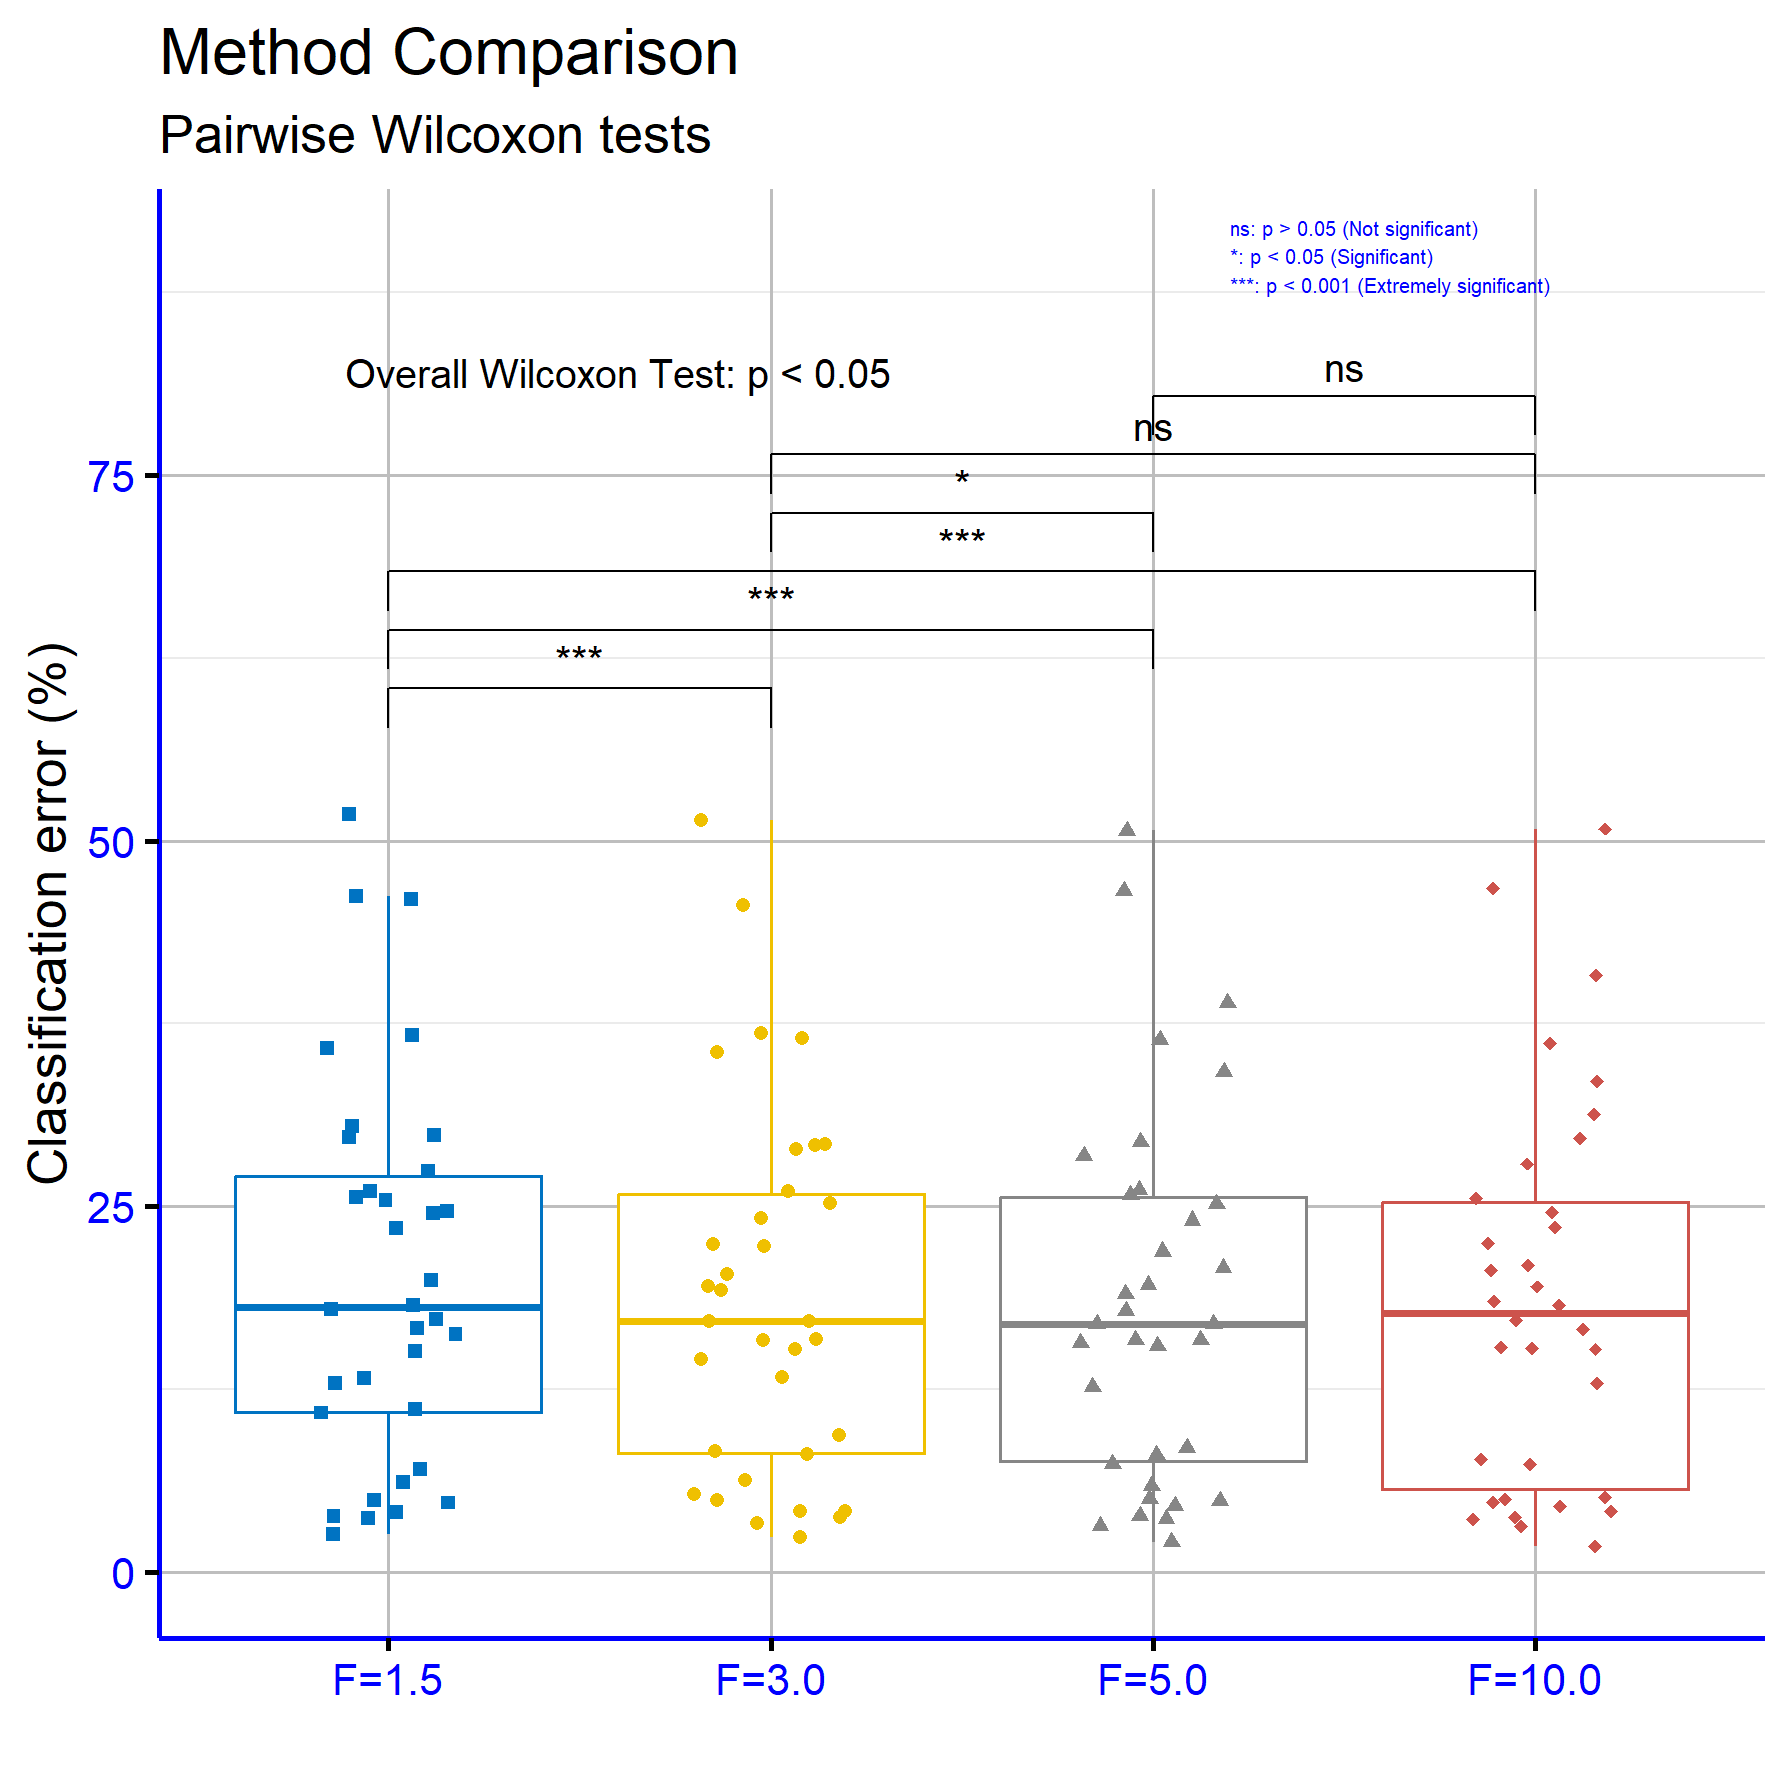
\includegraphics[scale=0.5]{img5}
\par\end{centering}
\caption{Statistical comparison for the experimental results by the application
of the proposed method with different values of parameter $F$. The
method was applied on the classification datasets.\protect\label{fig:statClassF}}

\end{figure}
Figure \ref{fig:statRegressionF} examines comparisons of parameter
$F$ for the regression datasets and shows no statistically significant
differences. The p-values for the comparisons $F=1.5$ vs $F=3.0$
($p=0.18$), $F=1.5$ vs $F=5.0$ ($p=0.15$), $F=1.5$ vs $F=10.0$
($p=0.21$), $F=3.0$ vs $F=5.0$ ($p=0.7$), $F=3.0$ vs $F=10.0$
($p=0.54$), and $F=5.0$ vs $F=10.0$ ($p=0.89$) indicate that variations
in the value of parameter $F$ do not significantly affect the model's
performance on the regression datasets. This may suggest greater stability
of the model to changes in this parameter compared to the classification
datasets.

\begin{figure}[H]
\begin{centering}
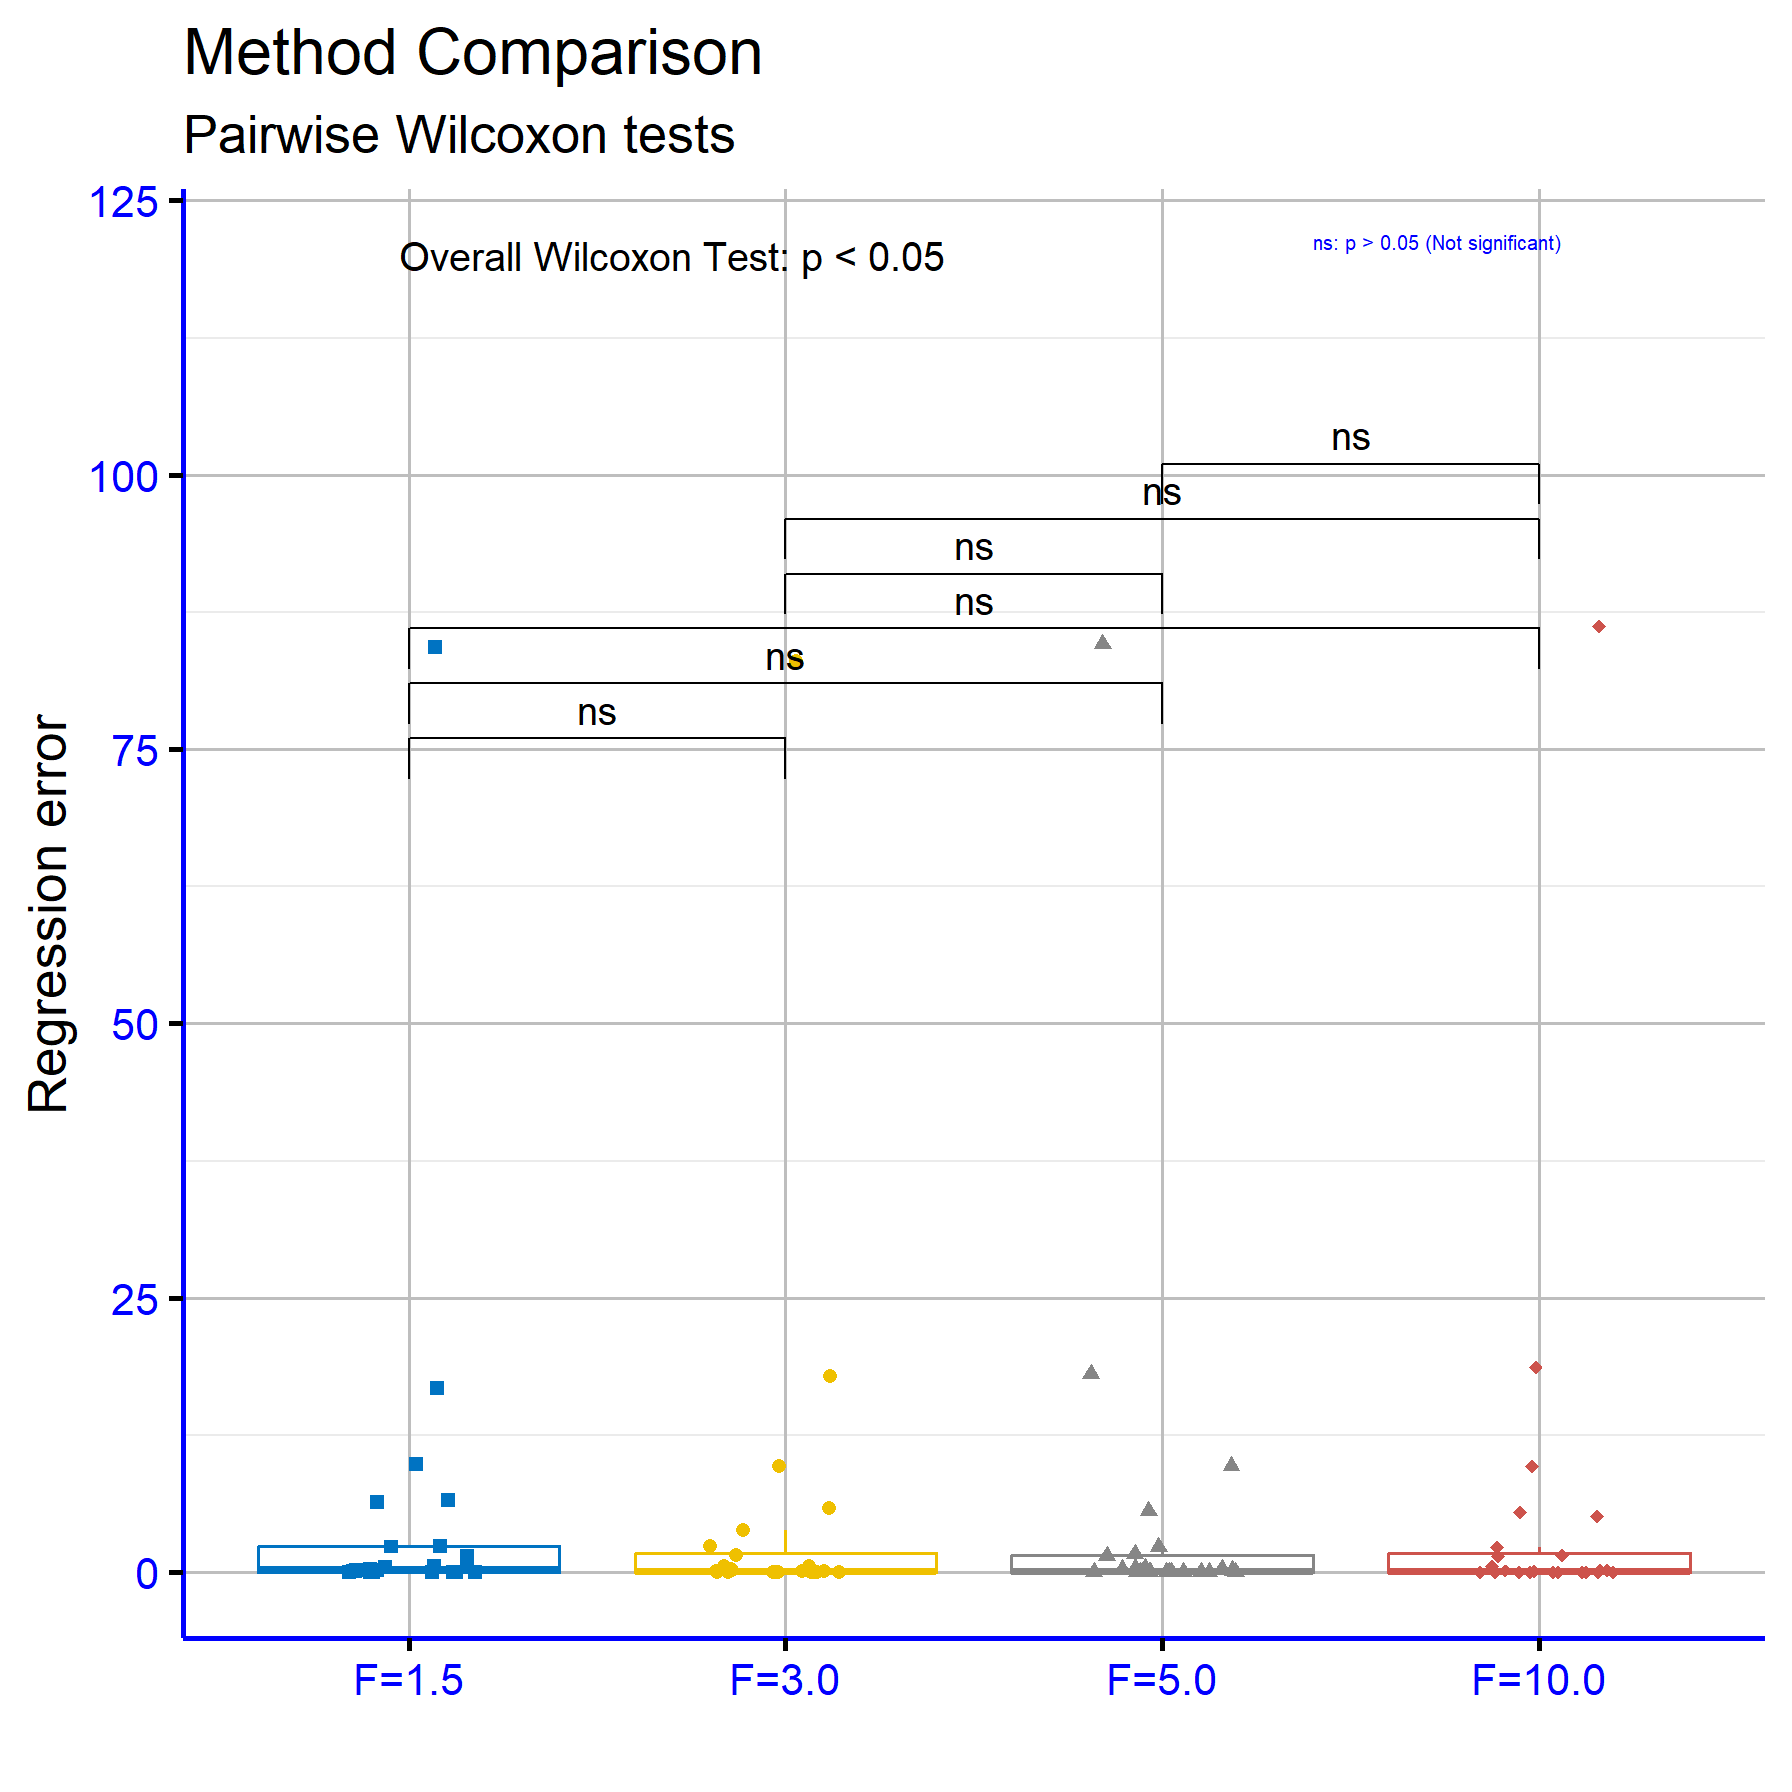
\includegraphics[scale=0.5]{img6}
\par\end{centering}
\caption{Statistical comparison for the obtained results by the application
of the proposed method to the regression datasets. For this experiment
different values of parameter $F$ were used.\protect\label{fig:statRegressionF}}

\end{figure}


\section{Conclusions \protect\label{sec:Conclusions}}

The article focuses on optimizing the parameter tuning process in
Radial Basis Function networks through a multidimensional and innovative
approach that combines techniques such as Simulated Annealing and
genetic algorithms. The proposed method surpasses traditional two-stage
approaches, where parameters are typically determined using fixed
processes like K-means clustering followed by a split between training
and validation phases. Instead, the article introduces a three-phase
process. In the first phase, initial parameter estimation is performed
using K-means, ensuring a stable starting point. In the second phase,
the application of Simulated Annealing provides an advanced mechanism
for exploring the parameter space, avoiding local minima and examining
a broader range of potential values. Finally, the third phase integrates
genetic algorithms, enabling the optimization of parameters based
on the model's actual performance. This process ensures a comprehensive
and adaptive approach, reducing the likelihood of overfitting and
numerical instability. The novelty of the method lies not only in
the three-phase process but also in the model's ability to adapt to
datasets with diverse characteristics, such as those involving complex
nonlinear relationships or multidimensional dependencies. Experimental
results demonstrate the method's superiority compared to traditional
techniques, such as BFGS, ADAM, NEAT, and RBF-KMEANS, achieving improvements
in terms of average error rates across both classification and regression
datasets.

The article's conclusions clearly highlight the superiority of the
proposed method. In classification datasets, the method achieves lower
average error rates, particularly when parameters $a$ and $F$ are
optimally configured. For instance, in classification datasets, the
parameter $F$ significantly influences performance, with $F=5.0$
proving to be the most effective value in many cases. In datasets
such as \textquotedbl Ionosphere\textquotedbl{} and \textquotedbl Wine,\textquotedbl{}
dramatic reductions in error rates are observed as the value of $F$
increases, emphasizing the importance of selecting this parameter
correctly. Similarly, in regression datasets, the proposed model demonstrates
exceptional performance, with notable examples including datasets
like \textquotedbl Abalone\textquotedbl{} and \textquotedbl Friedman,\textquotedbl{}
where the error decreases significantly compared to traditional techniques.
The \textquotedbl MB\textquotedbl{} dataset is particularly interesting,
as the use of Simulated Annealing contributed to a substantial performance
improvement, avoiding errors commonly encountered in traditional approaches.
Despite the generally positive results, there are cases where the
method's performance is suboptimal, such as in the \textquotedbl Segment\textquotedbl{}
dataset, indicating that the method is not universally generalizable
without adjustment to the characteristics of each dataset. The need
for further research on the parameters $a$ and $F$ becomes evident,
as these parameters critically impact performance across numerous
datasets.

For the future, the article proposes numerous directions for further
exploration and development. Initially, applying the method to more
diverse data categories, such as time series, image data, or even
genetic data, could broaden its application scope. Additionally, the
dynamic adjustment of parameters $a$ and $F$ during training, using
reinforcement learning techniques, could further enhance performance
by eliminating the need for manual tuning. Furthermore, integrating
the method into deep learning systems, such as Convolutional or Recurrent
Neural Networks, could lead to hybrid approaches that combine the
flexibility of RBF with the computational power of deep neural networks.
Moreover, investigating the robustness of the method in environments
with dynamic or imbalanced data could provide additional insights
into its generalizability. Finally, analyzing the method's performance
on big data and integrating it with technologies like distributed
processing or cloud computing could open new avenues, enabling its
scalability to larger-scale problems. The methodology proposed in
the article not only sets new standards for the performance of RBF
but also paves the way for further innovation in the field of machine
learning.

\vspace{6pt}


\authorcontributions{V.C. and I.G.T. conducted the experiments, employing several datasets
and provided the comparative experiments. D.T. and V.C. performed
the statistical analysis and prepared the manuscript. All authors
have read and agreed to the published version of the manuscript.}

\funding{This research received no external funding.}

\institutionalreview{Not applicable.}

\informedconsent{Not applicable. }

\informedconsent{Not applicable. }

\acknowledgments{This research has been financed by the European Union : Next Generation
EU through the Program Greece 2.0 National Recovery and Resilience
Plan , under the call RESEARCH -- CREATE -- INNOVATE, project name
“iCREW: Intelligent small craft simulator for advanced crew training
using Virtual Reality techniques\textquotedbl{} (project code:TAEDK-06195).
\quad{}}

\conflictsofinterest{The authors declare no conflict of interest.}

Not applicable.

\appendixtitles{no}

\appendixstart{}

\appendix

\begin{adjustwidth}{-\extralength}{0cm}{}


\reftitle{References}
\begin{thebibliography}{99}
\bibitem[(2006)]{physics_ml1} M. Mjahed, The use of clustering techniques
for the classification of high energy physics data, Nuclear Instruments
and Methods in Physics Research Section A: Accelerators, Spectrometers,
Detectors and Associated Equipment \textbf{559}, pp. 199-202, 2006.

\bibitem{physics_ml2}M Andrews, M Paulini, S Gleyzer, B Poczos, End-to-End
Event Classification of High-Energy Physics Data, Journal of Physics:
Conference Series \textbf{1085}, 2018.

\bibitem[(2006)]{astronomy_ml1}Viquar, M., Basak, S., Dasgupta, A.,
Agrawal, S., \& Saha, S. (2019). Machine learning in astronomy: A
case study in quasar-star classification. Emerging Technologies in
Data Mining and Information Security: Proceedings of IEMIS 2018, Volume
3, 827-836.

\bibitem[(2006)]{astronomy_ml2}Luo, S., Leung, A. P., Hui, C. Y.,
\& Li, K. L. (2020). An investigation on the factors affecting machine
learning classifications in gamma-ray astronomy. Monthly Notices of
the Royal Astronomical Society, 492(4), 5377-5390.

\bibitem[(2006)]{chemistry_ml1}P. He, C.J. Xu, Y.Z. Liang, K.T. Fang,
Improving the classification accuracy in chemistry via boosting technique,
Chemometrics and Intelligent Laboratory Systems 70, pp. 39-46, 2004.

\bibitem{chemistry_ml2}J.A. Aguiar, M.L. Gong, T.Tasdizen, Crystallographic
prediction from diffraction and chemistry data for higher throughput
classification using machine learning, Computational Materials Science
\textbf{173}, 109409, 2020.

\bibitem[(2006)]{med_ml1}S.S. Yadav, S.M. Jadhav, Deep convolutional
neural network based medical image classification for disease diagnosis.
J Big Data \textbf{6}, 113, 2019.

\bibitem{med_ml2}L. Qing, W. Linhong , D. Xuehai, A Novel Neural
Network-Based Method for Medical Text Classification, Future Internet
\textbf{11}, 255, 2019. 

\bibitem[(2006)]{econ_ml1}I. Kaastra, M. Boyd, Designing a neural
network for forecasting financial and economic time series, Neurocomputing
\textbf{10}, pp. 215-236, 1996.

\bibitem{econ_ml2}R. Hafezi, J. Shahrabi, E. Hadavandi, A bat-neural
network multi-agent system (BNNMAS) for stock price prediction: Case
study of DAX stock price, Applied Soft Computing \textbf{29}, pp.
196-210, 2015.

\bibitem[(2006)]{kmeans}MacQueen, J.: Some methods for classification
and analysis of multivariate observations, in: Proceedings of the
fifth Berkeley symposium on mathematical statistics and probability,
Vol. 1, No. 14, pp. 281-297, 1967. 

\bibitem[(2006)]{rbfface}M.J. Er, S. Wu, J. Lu, H.L. Toh, Face recognition
with radial basis function (RBF) neural networks, IEEE Transactions
on Neural Networks \textbf{13}, pp. 697-710, 2002.

\bibitem[(2006)]{rbfde1}Nam Mai-Duy, Thanh Tran-Cong, Numerical solution
of differential equations using multiquadric radial basis function
networks, Neural Networks 14, pp. 185-199, 2001.

\bibitem{rbfde2}N. Mai‐Duy, Solving high order ordinary differential
equations with radial basis function networks. Int. J. Numer. Meth.
Engng. \textbf{62}, pp. 824-852, 2005.

\bibitem[(2006)]{rbfstock}Shen, W., Guo, X., Wu, C., \& Wu, D. (2011).
Forecasting stock indices using radial basis function neural networks
optimized by artificial fish swarm algorithm. Knowledge-Based Systems,
24(3), 378-385.

\bibitem[(2006)]{rbfrobotics1}R. -J. Lian, Adaptive Self-Organizing
Fuzzy Sliding-Mode Radial Basis-Function Neural-Network Controller
for Robotic Systems, IEEE Transactions on Industrial Electronics \textbf{61},
pp. 1493-1503, 2014.

\bibitem{rbfrobotics2}M. Vijay, D. Jena, Backstepping terminal sliding
mode control of robot manipulator using radial basis functional neural
networks. Computers \& Electrical Engineering \textbf{67}, pp. 690-707,
2018.

\bibitem[(2006)]{rbf_dos1}U. Ravale, N. Marathe, P. Padiya, Feature
Selection Based Hybrid Anomaly Intrusion Detection System Using K
Means and RBF Kernel Function, Procedia Computer Science \textbf{45},
pp. 428-435, 2015.

\bibitem{rbf_dos2}M. Lopez-Martin, A. Sanchez-Esguevillas, J. I.
Arribas, B. Carro, Network Intrusion Detection Based on Extended RBF
Neural Network With Offline Reinforcement Learning, IEEE Access \textbf{9},
pp. 153153-153170, 2021.

\bibitem[(2006)]{rbfkernel}N. Benoudjit, M. Verleysen, On the Kernel
Widths in Radial-Basis Function Networks, Neural Processing Letters
\textbf{18}, pp. 139--154, 2003.

\bibitem[(2006)]{rbfkernel2}Oyang, Y. J., Hwang, S. C., Ou, Y. Y.,
Chen, C. Y., \& Chen, Z. W. (2005). Data classification with radial
basis function networks based on a novel kernel density estimation
algorithm. IEEE transactions on neural networks, 16(1), 225-236.

\bibitem[(2006)]{rbfinit1}Ros, F., Pintore, M., Deman, A., \& Chrétien,
J. R. (2007). Automatical initialization of RBF neural networks. Chemometrics
and intelligent laboratory systems, 87(1), 26-32.

\bibitem[(2006)]{rbfprun1}E. Ricci, R. Perfetti, Improved pruning
strategy for radial basis function networks with dynamic decay adjustment,
Neurocomputing \textbf{69}, pp. 1728-1732, 2006.

\bibitem[(2006)]{rbfprun2}Guang-Bin Huang, P. Saratchandran and N.
Sundararajan, A generalized growing and pruning RBF (GGAP-RBF) neural
network for function approximation, IEEE Transactions on Neural Networks
\textbf{16}, pp. 57-67, 2005.

\bibitem[(2006)]{rbfga1}Harpham, C., Dawson, C. W., \& Brown, M.
R. (2004). A review of genetic algorithms applied to training radial
basis function networks. Neural Computing \& Applications, 13, 193-201.

\bibitem[(2006)]{rbfga2}Sarimveis, H., Alexandridis, A., Mazarakis,
S., \& Bafas, G. (2004). A new algorithm for developing dynamic radial
basis function neural network models based on genetic algorithms.
Computers \& chemical engineering, 28(1-2), 209-217.

\bibitem[(2006)]{rbfpso1}Rani R, H. J., \& Victoire T, A. A. (2018).
Training radial basis function networks for wind speed prediction
using PSO enhanced differential search optimizer. PloS one, 13(5),
e0196871.

\bibitem[(2006)]{rbfpso2}Zhang, W., \& Wei, D. (2018). Prediction
for network traffic of radial basis function neural network model
based on improved particle swarm optimization algorithm. Neural Computing
and Applications, 29(4), 1143-1152.

\bibitem[(2006)]{rbfdiff1}Qasem, S. N., Shamsuddin, S. M., \& Zain,
A. M. (2012). Multi-objective hybrid evolutionary algorithms for radial
basis function neural network design. Knowledge-Based Systems, 27,
475-497.

\bibitem[(2006)]{rbfpar1}R. Yokota, L.A. Barba, M. G. Knepley, PetRBF
--- A parallel O(N) algorithm for radial basis function interpolation
with Gaussians, Computer Methods in Applied Mechanics and Engineering
\textbf{199}, pp. 1793-1804, 2010.

\bibitem{rbfpar2}C. Lu, N. Ma, Z. Wang, Fault detection for hydraulic
pump based on chaotic parallel RBF network, EURASIP J. Adv. Signal
Process. \textbf{2011}, 49, 2011.

\bibitem[(2006)]{siman1}L. Ingber, Very fast simulated re-annealing,
Mathematical and Computer Modelling \textbf{12}, pp. 967-973, 1989.

\bibitem[(2006)]{sa_resource}Aerts, J. C., \& Heuvelink, G. B. (2002).
Using simulated annealing for resource allocation. International Journal
of Geographical Information Science, 16(6), 571-587.

\bibitem[(2006)]{sa_portfolio}K. Ganesh, M. Punniyamoorthy, Optimization
of continuous-time production planning using hybrid genetic algorithms-simulated
annealing, Int J Adv Manuf Technol \textbf{26}, pp. 148--154, 2005.

\bibitem[(2006)]{sa_solar}El-Naggar, K. M., AlRashidi, M. R., AlHajri,
M. F., \& Al-Othman, A. K. (2012). Simulated annealing algorithm for
photovoltaic parameters identification. Solar Energy, 86(1), 266-274.

\bibitem[(2006)]{sa_biology}Dupanloup, I., Schneider, S., \& Excoffier,
L. (2002). A simulated annealing approach to define the genetic structure
of populations. Molecular ecology, 11(12), 2571-2581.

\bibitem[(2007)]{kaelo}P. Kaelo, M.M. Ali, Integrated crossover rules
in real coded genetic algorithms, European Journal of Operational
Research \textbf{176}, pp. 60-76, 2007.

\bibitem{UCL}M. Kelly, R. Longjohn, K. Nottingham, The UCI Machine
Learning Repository. 2023. Available online: https://archive.ics.uci.edu
(accessed on 20 September 2023).

\bibitem{Keel}J. Alcalá-Fdez, A. Fernandez, J. Luengo, J. Derrac,
S. García, L. Sánchez, F. Herrera. KEEL Data-Mining Software Tool:
Data Set Repository, Integration of Algorithms and Experimental Analysis
Framework. Journal of Multiple-Valued Logic and Soft Computing 17,
pp. 255-287, 2011.

\bibitem[(2018)]{Alcohol}Tzimourta, K.D.; Tsoulos, I.; Bilero, I.T.;
Tzallas, A.T.; Tsipouras, M.G.; Giannakeas, N. Direct Assessment of
Alcohol Consumption in Mental State Using Brain Computer Interfaces
and Grammatical Evolution. Inventions 2018, 3, 51.

\bibitem{appendicitis}Weiss, Sholom M. and Kulikowski, Casimir A.,
Computer Systems That Learn: Classification and Prediction Methods
from Statistics, Neural Nets, Machine Learning, and Expert Systems,
Morgan Kaufmann Publishers Inc, 1991.

\bibitem[Quinlan(2018)]{australian}J.R. Quinlan, Simplifying Decision
Trees. International Journal of Man-Machine Studies \textbf{27}, pp.
221-234, 1987. 

\bibitem{balance}T. Shultz, D. Mareschal, W. Schmidt, Modeling Cognitive
Development on Balance Scale Phenomena, Machine Learning \textbf{16},
pp. 59-88, 1994.

\bibitem[(2004)]{cleveland1}Z.H. Zhou,Y. Jiang, NeC4.5: neural ensemble
based C4.5,\textquotedbl{} in IEEE Transactions on Knowledge and Data
Engineering \textbf{16}, pp. 770-773, 2004.

\bibitem{cleveland2}R. Setiono , W.K. Leow, FERNN: An Algorithm for
Fast Extraction of Rules from Neural Networks, Applied Intelligence
\textbf{12}, pp. 15-25, 2000.

\bibitem[(1998)]{dermatology}G. Demiroz, H.A. Govenir, N. Ilter,
Learning Differential Diagnosis of Eryhemato-Squamous Diseases using
Voting Feature Intervals, Artificial Intelligence in Medicine. \textbf{13},
pp. 147--165, 1998.

\bibitem[(1977)]{hayes-roth}B. Hayes-Roth, B., F. Hayes-Roth. Concept
learning and the recognition and classification of exemplars. Journal
of Verbal Learning and Verbal Behavior \textbf{16}, pp. 321-338, 1977.

\bibitem[(1997)]{heart}I. Kononenko, E. Šimec, M. Robnik-Šikonja,
Overcoming the Myopia of Inductive Learning Algorithms with RELIEFF,
Applied Intelligence \textbf{7}, pp. 39--55, 1997.

\bibitem[(2002)]{housevotes}R.M. French, N. Chater, Using noise to
compute error surfaces in connectionist networks: a novel means of
reducing catastrophic forgetting, Neural Comput. \textbf{14}, pp.
1755-1769, 2002.

\bibitem[(2004)]{ion1}J.G. Dy , C.E. Brodley, Feature Selection for
Unsupervised Learning, The Journal of Machine Learning Research \textbf{5},
pp 845--889, 2004.

\bibitem{ion2}S. J. Perantonis, V. Virvilis, Input Feature Extraction
for Multilayered Perceptrons Using Supervised Principal Component
Analysis, Neural Processing Letters \textbf{10}, pp 243--252, 1999.

\bibitem[(2002)]{liver1} J. Garcke, M. Griebel, Classification with
sparse grids using simplicial basis functions, Intell. Data Anal.
\textbf{6}, pp. 483-502, 2002.

\bibitem{liver2}J. Mcdermott, R.S. Forsyth, Diagnosing a disorder
in a classification benchmark, Pattern Recognition Letters \textbf{73},
pp. 41-43, 2016.

\bibitem[(2002)]{lymography}G. Cestnik, I. Konenenko, I. Bratko,
Assistant-86: A Knowledge-Elicitation Tool for Sophisticated Users.
In: Bratko, I. and Lavrac, N., Eds., Progress in Machine Learning,
Sigma Press, Wilmslow, pp. 31-45, 1987. 

\bibitem[(2007)]{mammographic}M. Elter, R. Schulz-Wendtland, T. Wittenberg,
The prediction of breast cancer biopsy outcomes using two CAD approaches
that both emphasize an intelligible decision process, Med Phys. \textbf{34},
pp. 4164-72, 2007.

\bibitem[(2007)]{parkinsons1}M.A. Little, P.E. McSharry, S.J Roberts
et al, Exploiting Nonlinear Recurrence and Fractal Scaling Properties
for Voice Disorder Detection. BioMed Eng OnLine \textbf{6}, 23, 2007.

\bibitem{parkinsons2}M.A. Little, P.E. McSharry, E.J. Hunter, J.
Spielman, L.O. Ramig, Suitability of dysphonia measurements for telemonitoring
of Parkinson's disease. IEEE Trans Biomed Eng. \textbf{56}, pp. 1015-1022,
2009.

\bibitem[(2007)]{pima}J.W. Smith, J.E. Everhart, W.C. Dickson, W.C.
Knowler, R.S. Johannes, Using the ADAP learning algorithm to forecast
the onset of diabetes mellitus, In: Proceedings of the Symposium on
Computer Applications and Medical Care IEEE Computer Society Press,
pp.261-265, 1988.

\bibitem[(2007)]{popfailures}D.D. Lucas, R. Klein, J. Tannahill,
D. Ivanova, S. Brandon, D. Domyancic, Y. Zhang, Failure analysis of
parameter-induced simulation crashes in climate models, Geoscientific
Model Development \textbf{6}, pp. 1157-1171, 2013.

\bibitem[(2007)]{regions2}N. Giannakeas, M.G. Tsipouras, A.T. Tzallas,
K. Kyriakidi, Z.E. Tsianou, P. Manousou, A. Hall, E.C. Karvounis,
V. Tsianos, E. Tsianos, A clustering based method for collagen proportional
area extraction in liver biopsy images (2015) Proceedings of the Annual
International Conference of the IEEE Engineering in Medicine and Biology
Society, EMBS, 2015-November, art. no. 7319047, pp. 3097-3100. 

\bibitem[(2007)]{saheart}T. Hastie, R. Tibshirani, Non-parametric
logistic and proportional odds regression, JRSS-C (Applied Statistics)
\textbf{36}, pp. 260--276, 1987.

\bibitem{segment}M. Dash, H. Liu, P. Scheuermann, K. L. Tan, Fast
hierarchical clustering and its validation, Data \& Knowledge Engineering
\textbf{44}, pp 109--138, 2003.

\bibitem{sonar}Gorman, R.P.; Sejnowski, T.J. Analysis of Hidden Units
in a Layered Network Trained to Classify Sonar Targets. Neural Netw.
1988, 1, 75--89.

\bibitem{student}P. Cortez, A. M. Gonçalves Silva, Using data mining
to predict secondary school student performance, In Proceedings of
5th FUture BUsiness TEChnology Conference (FUBUTEC 2008) (pp. 5--12).
EUROSIS-ETI, 2008.

\bibitem[(2009)]{transfusion}I-Cheng Yeh, King-Jang Yang, Tao-Ming
Ting, Knowledge discovery on RFM model using Bernoulli sequence, Expert
Systems with Applications \textbf{36}, pp. 5866-5871, 2009.

\bibitem{wdbc}W.H. Wolberg, O.L. Mangasarian, Multisurface method
of pattern separation for medical diagnosis applied to breast cytology,
Proc Natl Acad Sci U S A. \textbf{87}, pp. 9193--9196, 1990.

\bibitem{wine1}M. Raymer, T.E. Doom, L.A. Kuhn, W.F. Punch, Knowledge
discovery in medical and biological datasets using a hybrid Bayes
classifier/evolutionary algorithm. IEEE transactions on systems, man,
and cybernetics. Part B, Cybernetics : a publication of the IEEE Systems,
Man, and Cybernetics Society, \textbf{33} , pp. 802-813, 2003.

\bibitem{wine2}P. Zhong, M. Fukushima, Regularized nonsmooth Newton
method for multi-class support vector machines, Optimization Methods
and Software \textbf{22}, pp. 225-236, 2007.

\bibitem[(2007)]{eeg1}R. G. Andrzejak, K. Lehnertz, F.Mormann, C.
Rieke, P. David, and C. E. Elger, “Indications of nonlinear deterministic
and finite-dimensional structures in time series of brain electrical
activity: dependence on recording region and brain state,” Physical
Review E, vol. 64, no. 6, Article ID 061907, 8 pages, 2001. 

\bibitem{eeg2}A. T. Tzallas, M. G. Tsipouras, and D. I. Fotiadis,
“Automatic Seizure Detection Based on Time-Frequency Analysis and
Artificial Neural Networks,” Computational Intelligence and Neuroscience,
vol. 2007, Article ID 80510, 13 pages, 2007. doi:10.1155/2007/80510.

\bibitem[(2007)]{zoo}M. Koivisto, K. Sood, Exact Bayesian Structure
Discovery in Bayesian Networks, The Journal of Machine Learning Research\textbf{
5}, pp. 549--573, 2004.

\bibitem[(2018)]{abalone}Nash, W.J.; Sellers, T.L.; Talbot, S.R.;
Cawthor, A.J.; Ford, W.B. The Population Biology of Abalone (\_Haliotis\_
species) in Tasmania. I. Blacklip Abalone (\_H. rubra\_) from the
North Coast and Islands of Bass Strait, Sea Fisheries Division; Technical
Report No. 48; Department of Primary Industry and Fisheries, Tasmania:
Hobart, Australia, 1994; ISSN 1034-3288

\bibitem[(2007)]{airfoil}Brooks, T.F.; Pope, D.S.; Marcolini, A.M.
Airfoil Self-Noise and Prediction. Technical Report, NASA RP-1218.
July 1989. Available online: https://ntrs.nasa.gov/citations/19890016302
(accessed on 5 March 2025).

\bibitem{BK}J.S. Simonoff, Smooting Methods in Statistics, Springer
- Verlag, 1996.

\bibitem{concrete}I.Cheng Yeh, Modeling of strength of high performance
concrete using artificial neural networks, Cement and Concrete Research.
\textbf{28}, pp. 1797-1808, 1998. 

\bibitem{housing}D. Harrison and D.L. Rubinfeld, Hedonic prices and
the demand for clean ai, J. Environ. Economics \& Management \textbf{5},
pp. 81-102, 1978.

\bibitem{friedman}Friedman, J. (1991): Multivariate Adaptative Regression
Splines. Annals of Statistics, 19:1, 1-{}-141. 

\bibitem[(2018)]{ntdataset}Mackowiak, P.A., Wasserman, S.S., Levine,
M.M., 1992. A critical appraisal of 98.6 degrees f, the upper limit
of the normal body temperature, and other legacies of Carl Reinhold
August Wunderlich. J. Amer. Med. Assoc. 268, 1578--1580

\bibitem{pydataset}R.D. King, S. Muggleton, R. Lewis, M.J.E. Sternberg,
Proc. Nat. Acad. Sci. USA \textbf{89}, pp. 11322--11326, 1992. 

\bibitem[(2007)]{powell}M.J.D Powell, A Tolerant Algorithm for Linearly
Constrained Optimization Calculations, Mathematical Programming \textbf{45},
pp. 547-566, 1989. 

\bibitem[(2007)]{nn1}C. Bishop, Neural Networks for Pattern Recognition,
Oxford University Press, 1995.

\bibitem{nn2}G. Cybenko, Approximation by superpositions of a sigmoidal
function, Mathematics of Control Signals and Systems \textbf{2}, pp.
303-314, 1989.

\bibitem[(2007)]{adam}D. P. Kingma, J. L. Ba, ADAM: a method for
stochastic optimization, in: Proceedings of the 3rd International
Conference on Learning Representations (ICLR 2015), pp. 1--15, 2015.

\bibitem[(2007)]{neat}K. O. Stanley, R. Miikkulainen, Evolving Neural
Networks through Augmenting Topologies, Evolutionary Computation \textbf{10},
pp. 99-127, 2002.

\bibitem[(2007)]{genrbf}S. Ding, L. Xu, C. Su et al, An optimizing
method of RBF neural network based on genetic algorithm. Neural Comput
\& Applic 21, pp. 333--336, 2012.

\end{thebibliography}
%%%%%%%%%%%%%%%%%%%%%%%%%%%%%%%%%%%%%%%%%%
%% for journal Sci
%\reviewreports{\\
%Reviewer 1 comments and authors' response\\
%Reviewer 2 comments and authors' response\\
%Reviewer 3 comments and authors' response
%}
%%%%%%%%%%%%%%%%%%%%%%%%%%%%%%%%%%%%%%%%%%

\PublishersNote{}

\end{adjustwidth}{}
\end{document}
